\chapter{Auswertung}

In diesem Kapitel soll das entwickelte System einer Auswertung unterzogen werden.
Im ersten Abschnitt soll zunächst das das verwendete Werkzeug \textit{JMH} sowie 
die allgemeine Durchführung der Tests beschrieben werden. Im zweiten Abschnitt 
folgen dann die einzelnen Tests sowie deren Auswertungen.

Die Auswertung erfolgt von Laufzeit Benchmarks. Dabei wird die Laufzeit von 
optimierten Methoden vor und nach der Optimierung durch das System gemessen und 
diese Ergebnisse miteinander verglichen. Darüber hinaus werden diese Ergebnisse 
anhand der Ausgabe des Systems begründet.

\section{Vorraussetzungen}

\subsection{Java Microbenchmarking Harness}

Microbenchmarks sind auf der JVM schwierig zu Erstellen. Das liegt vor allem 
an der \textit{Just-In-Time} Kompilierung von Java Bytecode. Die JVM stellt 
während der Laufzeit eines Programms fest, welche Abschnitte des Bytecodes 
häufig ausgeführt werden und kompiliert diese Teile dynamisch zu Maschinen Code.
Diese Kompilierung kann auch wieder rückgängig gemacht werden, wenn der übersetzte
Abschnitt nicht mehr so häufig oder in einem anderen Kontext verwendet wird. Zusätzlich 
erschwert die nicht deterministische Garbage Collection, während der 
Laufzeit, konsistente und aussagekräftige Ergebnisse.

Um diesen Problemen zu begegnen wurde das Projekt JMH verwendet. Das \textit{Java Benchmarking Harness} 
(kurz JMH) ist ein Projekt innerhalb des OpenJDKs. Es dient der Unterstützung der 
Erstellung und Ausführung von Java Microbenchmarks. Das Framework lässt sich in 
den Maven Build integrieren und bietet eine annotationsbasierte Konfiguration 
für die in Java geschriebenen Benchmarks. Zu messende Benchmarks werden als Methoden 
in einer oder mehreren Java Klassen geschrieben, die eben jenen Code ausführen dessen Ausführungszeit 
gemessen werden soll. 

\subsection{Test Durchführungen}

Alle Messungen wurden mit dem im vorherigen Abschnitt vorgestellten JMH durchgeführt. 
Gemessen werden soll die Ausführungszeit einer Methodenausführung im originalen, sowie
im Zustand nach der Anwendung des Systems auf diese Methode. Da es nicht möglich ist,
dass dieselbe Klasse, welche die optimierte Methode bereitstellt, zweimal (die originale 
sowie die optimierte Variante) im Klassenpfad aufzuführen, müssen die Messungen
jeweils für den originalen als auch den optimierten Methoden Aufruf separat durchgeführt werden.
Diese Messungen fanden auf einem von der Universität bereit gestellten Rechner statt,
der für Benchmarks zur Verfügung stand. 

Für alle Tests wurden in einem Thread 10 Durchläufen durchgeführt. Ein Durchlauf setzt
sich dabei aus Aufwärm- sowie einer Messphasen von jeweils 20 Iterationen zusammen. 
Daher existieren für jede Messung 200 Ergebnisse. Eine Iteration misst die Anzahl von 
Methoden Aufrufen in einer Sekunde und rechnet diesen Wert in einen Zeitwert um. 

Als Test-Programme wurde zum eine eigens zum Testen geschriebene Methode verwendet, 
sowie Xalan, ein freier XSLT-Prozessor der Apache Software Foundation. Beide Programme
wurden als Eingabe für das in dieser Arbeit beschriebene System verwendet und die
Ausgabe für diese Auswertung verwendet.

Die Benchmarks befinden sich in dem Unterprojekt \textit{jmh-benchmarks} welches als
Maven Eigenschaft den Pfad zum Xalan bzw. ExampleParser jar erwartet und diese
Bibliothek in den Klassenpfad aufnimmt. So wird entsprechend der Parameters ein
Benchmark entweder für die normale oder für die optimierte Variante des Java Archivs
gebaut. 

Für die automatische Auswertung der Ergebnisse wurde ein Skript geschrieben, dass die 
folgenden Schritte jeweils für die normale, als auch für die optimierte Variante ausführt:

\begin{enumerate}
	\item stößt die Maven Bauvorgänge für die beiden JMH-Benchmark Projekte an
	\item führt die resultierenden Benchmarks aus
	\item übergibt die Ausgabedatei einem R Skript um die Boxplots zu erzeugen. 
\end{enumerate}

Alle Benchmarks wurden mittels einer Oracle JVM in der Version 7 ausgeführt. 

\section{Benchmarks}

In diesem Abschnitt sollen sowohl die Ergebnisse der Messungen beschrieben, als auch 
anhand der Ergebnisse des Systems erläutert werden.

\subsection{Example Parser}

Der \textit{Example Parser} ist ein eigens für die Auswertung geschriebene Methode.
Diese soll die Möglichkeit darstellen, dass Optimierungen mit dem in hier beschriebenen
System möglich sind. Der Code stellt sich dabei wie folgt dar:

\begin{figure}[H]
	\begin{lstlisting}[language=Java]
	public String parse(String line) {
		StringBuilder result = new StringBuilder();

		for (int i = 0; i + 1 < line.length(); i+=2) {
			result.append(line.substring(i, i + 1));
		}

		return result.toString();
	}
	\end{lstlisting} 
	\caption{Example Parser}
\end{figure}

Wie dem Code zu entnehmen ist, wird hier die Methode \texttt{substring()} in 
Verbindung mit dem \texttt{StringBuilder} verwendet. Dieser Methode ist daher
optimal für die beiden verwendeten TypeLabels, wie sie in \ref{stringLabels} 
beschrieben sind. 

Aufgerufen wurde diese Methode in einem Benchmark mit einem 112 langen String. Die 
Boxplots in Abbildung \ref{bp:exampleBench} zeigen die Dauer der Ausführung
vor und nach der Optimierung durch das System. 

\begin{figure}[H]
	\centering
	\centerline{
		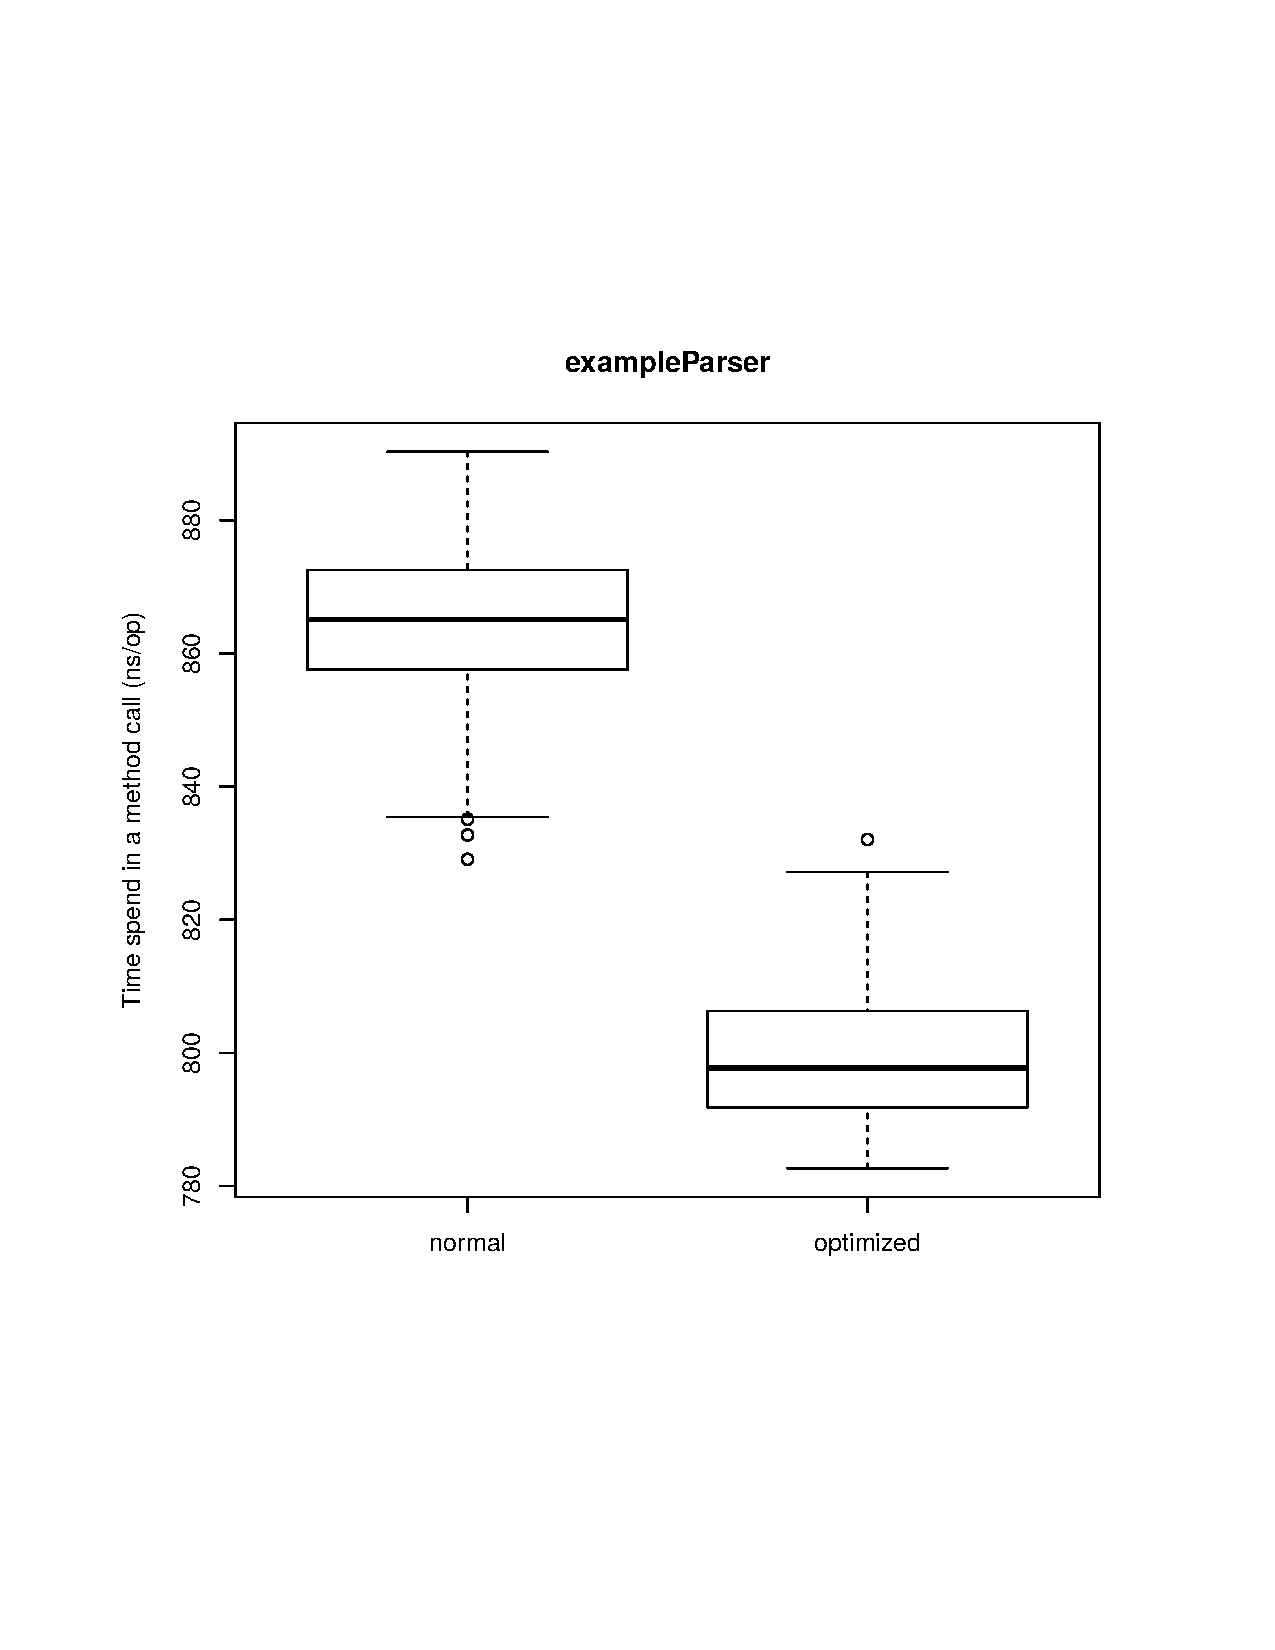
\includegraphics[trim=0mm 60mm 20mm 50mm,scale=0.50]{pictures/boxplot_exampleParser.pdf}
		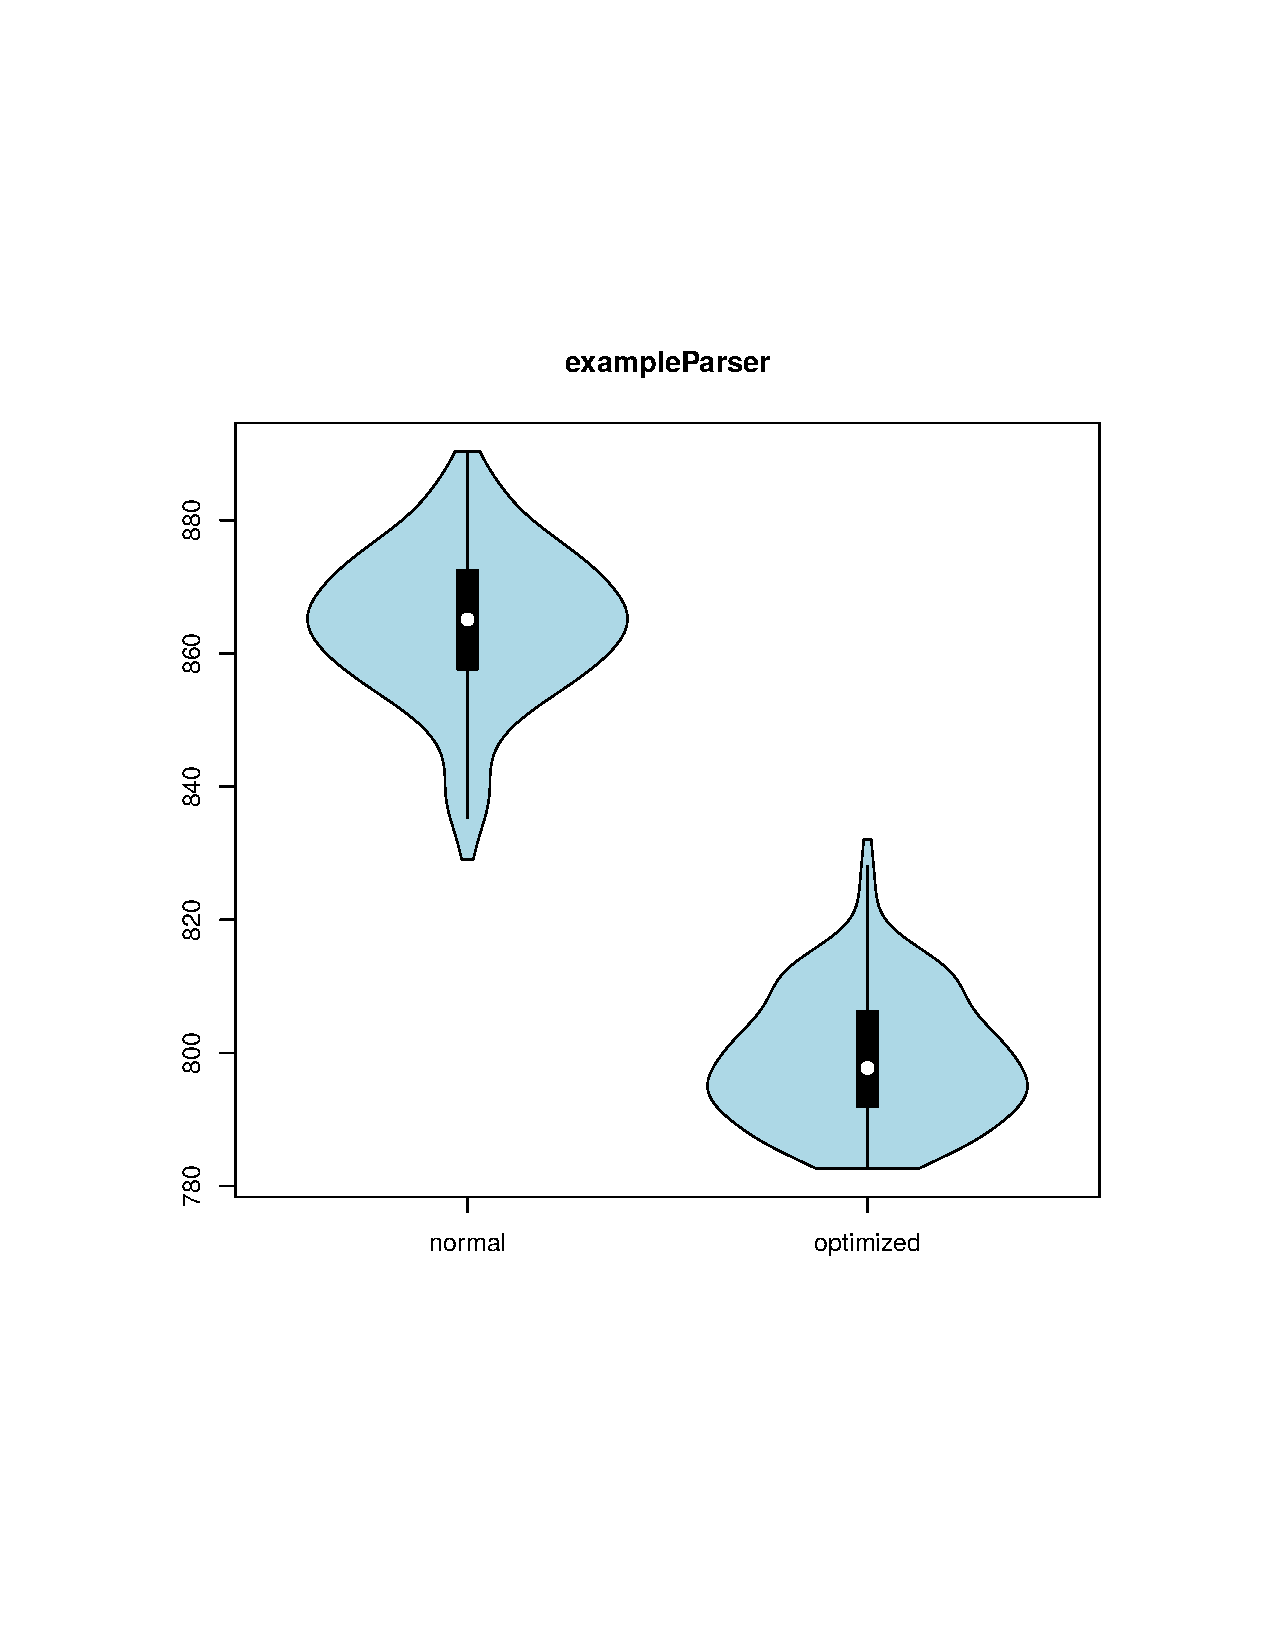
\includegraphics[trim=20mm 60mm 0mm 50mm,scale=0.50]{pictures/vioplot_exampleParser.pdf}
	}

	
	\begin{table}[H]
	\centering
		\begin{tabular}{|l|r|r|r|}
			\hline
		   		 	  & Mittelwert & Median & \bf{$\pm$ $0,1\%$} \\
		 	\hline
		 	\hline
		 	normal    & 864,41 & 865,10 & 2,689 \\ 
		  	optimiert & 799,14 & 797,72 & 2,295 \\
		  	\hline
		  	
		\end{tabular}
	\end{table}

	\caption{Ergebnis des Example Parser Benchmark}\label{bp:exampleBench}
\end{figure}


\subsubsection{Auswertung}

Aufgrund der optimalen Abstimmung der beiden optimierten Typen \texttt{SubstringString} und
\texttt{StringListBuilder} aufeinander, können die beiden Referenzen auch ohne irgendwelche 
Konvertierungen miteinander innerhalb der Methode koexistieren. Dies führt dazu, dass
erstellte \texttt{SubstringString} Referenzen direkt dem optimierten Stringbuilder übergeben
werden können. 

Dieser Benchmark soll zeigen, dass eine Optimierung, wenn auch nur für eine eigens dafür 
entwickelte Methode möglich ist. In den folgenden Benchmarks werden realitätsnahe Methoden für 
den Test des System verwendet.
 
\subsection{Xalan}

Zur Auswertung des Systems wurde der freie XSLT-Prozessor XALAN verwendet. Diese lag in Form 
eines Java Archivs vor, dass aus dem Quellcode der Version 2.7.2 gebaut wurde. 

Um geeignete Methoden für die Benchmarks zu finden, wurden die Anzahl der \texttt{substring(..)}
Aufrufe pro \texttt{*.java} Datei gezählt und diese Kandidaten nach absteigender Anzahl sortiert.
In diesen Kandidaten wurden diejenigen 4 Methoden als Tests verwendet, welche die meisten 
Aufrufe besaßen und auch ohne größeren Aufwand (öffentliche Methoden in wenig komplexen Objekten 
oder statisch) aus der Benchmark Methode aufrufbar waren. So viel die Wahl auf die folgenden 
Methoden:

\begin{description}
	\item [\texttt{org.apache.xalan.xsltc.runtime.BasisLibrary.checkAttribQName(java.lang.String)}]
		Prüft ob der gegebene XML-Attribut Name syntaktisch valide ist.
	\item [\texttt{org.apache.xml.utils.URI.new(java.lang.String)}]
		Erzeugt ein neues URI Objekt. 
	\item [\texttt{org.apache.xpath.objects.XNumber.str()}]
		Erstellt eine String Repräsentation des XNumber Objekts.
	\item [\texttt{javax.xml.xpath.XPath.compile(java.lang.String)}]
		Kompiliert den gegebenen XPath Ausdruck in ein auswertbares XPath-Objekt.
		
		Die eigentlich identifizierte Methode war \texttt{tokenize} des verwendeten 
		Lexers. Da dieser aber die Sichtbarkeit package-private
		besitzt wurde den kompletten Use Case, in dem dieser Lexer verwendet wird, 
		zu benutzen.
\end{description}

Als Eingaben dienten Werte, die der im Projekt enthaltenen Beispiel XML Dateien entnommen wurden 
und daher einen möglichst realen Ausführungskontext darstellen.

\subsubsection{checkAttribQName}

Diese Funktion prüft die syntaktische Validität eines XSLT-Attribut Namens. Dabei wird 
der Name anhand der ersten beiden ":" getrennt, was mit Hilfe der \texttt{substring} Methode
geschieht. 

Aufgerufen wurde diese Methode mit dem Wert "xmlns:redirect". Die folgende Abbildung zeigt 
die Ergebnisse der Messung.

\begin{figure}[H]
	\centering

	\centerline{
		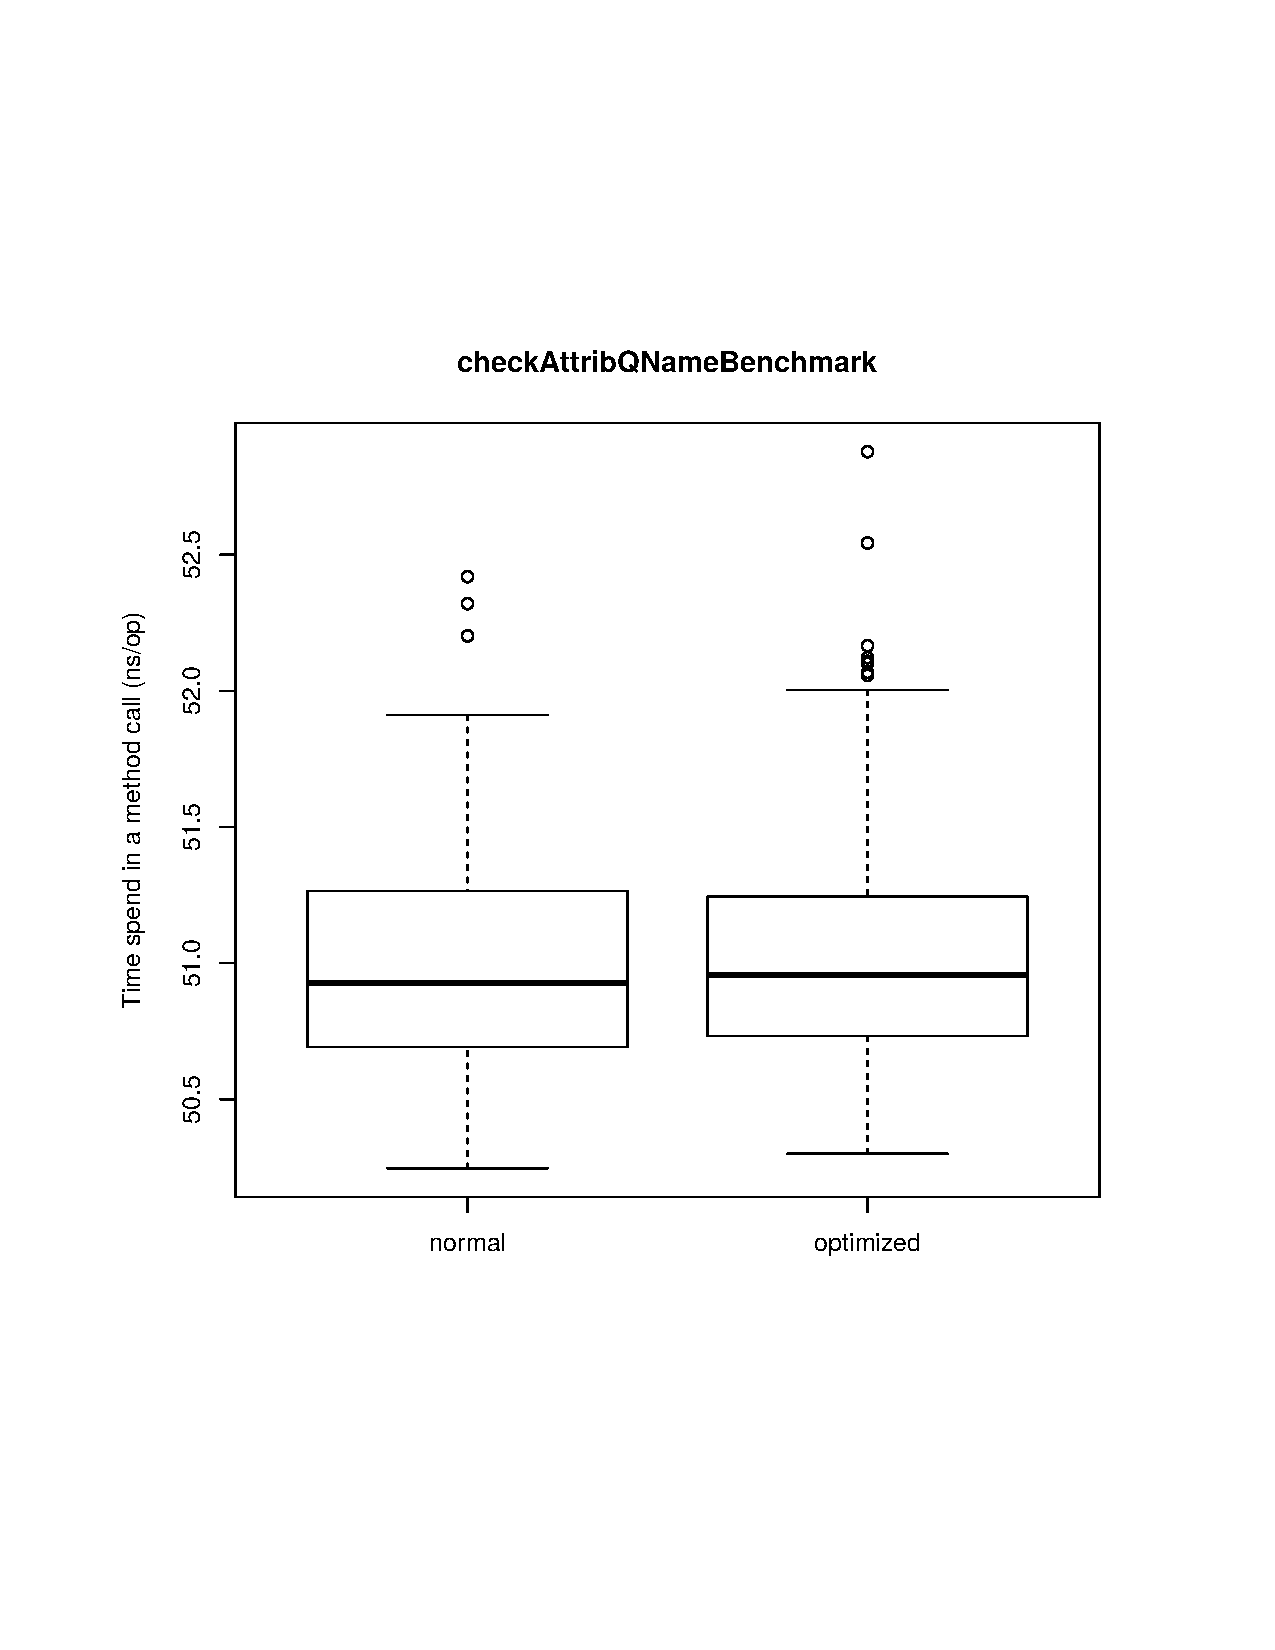
\includegraphics[trim=0mm 60mm 20mm 50mm,scale=0.50]{pictures/boxplot_checkAttribQName.pdf}
		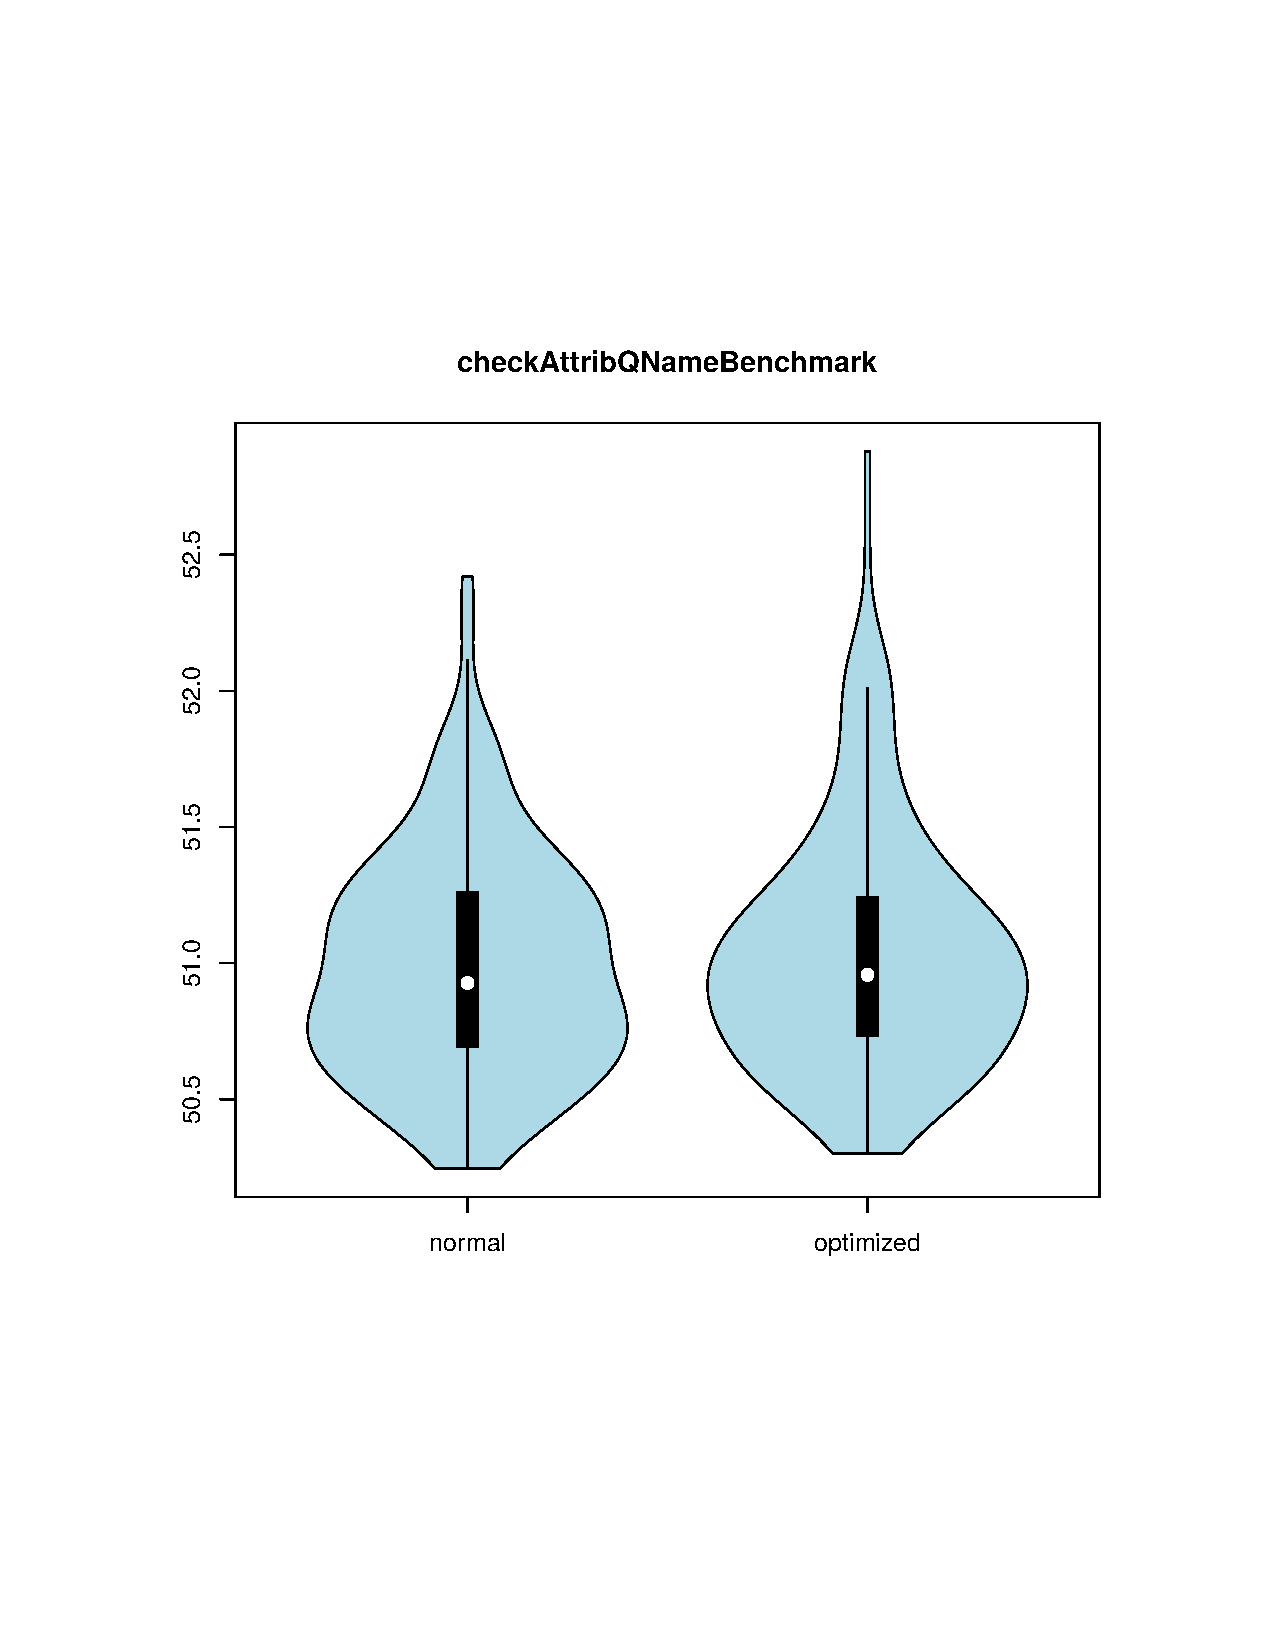
\includegraphics[trim=20mm 60mm 0mm 50mm,scale=0.50]{pictures/vioplot_checkAttribQName.pdf}
	}

	\begin{table}[H]
	\centering
		\begin{tabular}{|l|r|r|r|}
			\hline
		   		 	  & Mittelwert & Median & \bf{$\pm$ $0,1\%$} \\
		 	\hline
		 	\hline
		  	normal & 50,99 & 50,92 & 0,104 \\
		 	optimiert & 51,03 & 50,96 & 0,108 \\ 
		  	\hline
		  	
		\end{tabular}
	\end{table}

	\caption{Ergebnis des checkAttribQName Benchmark}\label{bp:checkAttrBench}
\end{figure}

\paragraph{Auswertung}

Die optimierte Referenz wird als Parameter an die Methode übergeben. Also beginnt mit diesem 
Parameter Knoten die Bubble für diese Referenz und sie wird direkt zu Beginn in eine
optimierten \texttt{SubstringString} konvertiert. Allerdings werden in den folgenden beiden 
Zeilen die auf dieser Referenz die Positionen der Doppelpunkte ermittelt. Diese Methoden
werden aber nicht von dem optimierten Typ angeboten, was dazu führt, dass an beiden dieser 
Stellen eine Rückkonvertierung zum originalen Typ stattfinden muss. 

Dieser zusätzliche Aufwand sorgt dafür, dass die Optimierung des \texttt{substring} Aufrufs
durch die Konvertierungen wieder ausgeglichen wird. 

\subsubsection{instantiateURI}

Bei dieser Methode handelt es sich um den Konstruktor der Klasse\\ \texttt{org.apache.xml.utils.URI}.
Dieser erwartet einen String, der die zu repräsentierende URI enthält. Der Konstruktor teilt
die übergebene Zeichenkette in semantische Bausteine, wie das Protokoll, die Domain oder den Pfad.
Zu diesem wird die Methode \texttt{substring} wiederholt auf den übergebenen String angewendet. 

Die Messung wurde mit dem Wert "http://xml.apache.org/xalan-j/apidocs/
javax/xml/transform/package-summary.html" durchgeführt. Die folgende Abbildung präsentiert 
die Ergebnisse dieses Benchmarks.

\begin{figure}[H]
	\centering
	
	\centerline{
		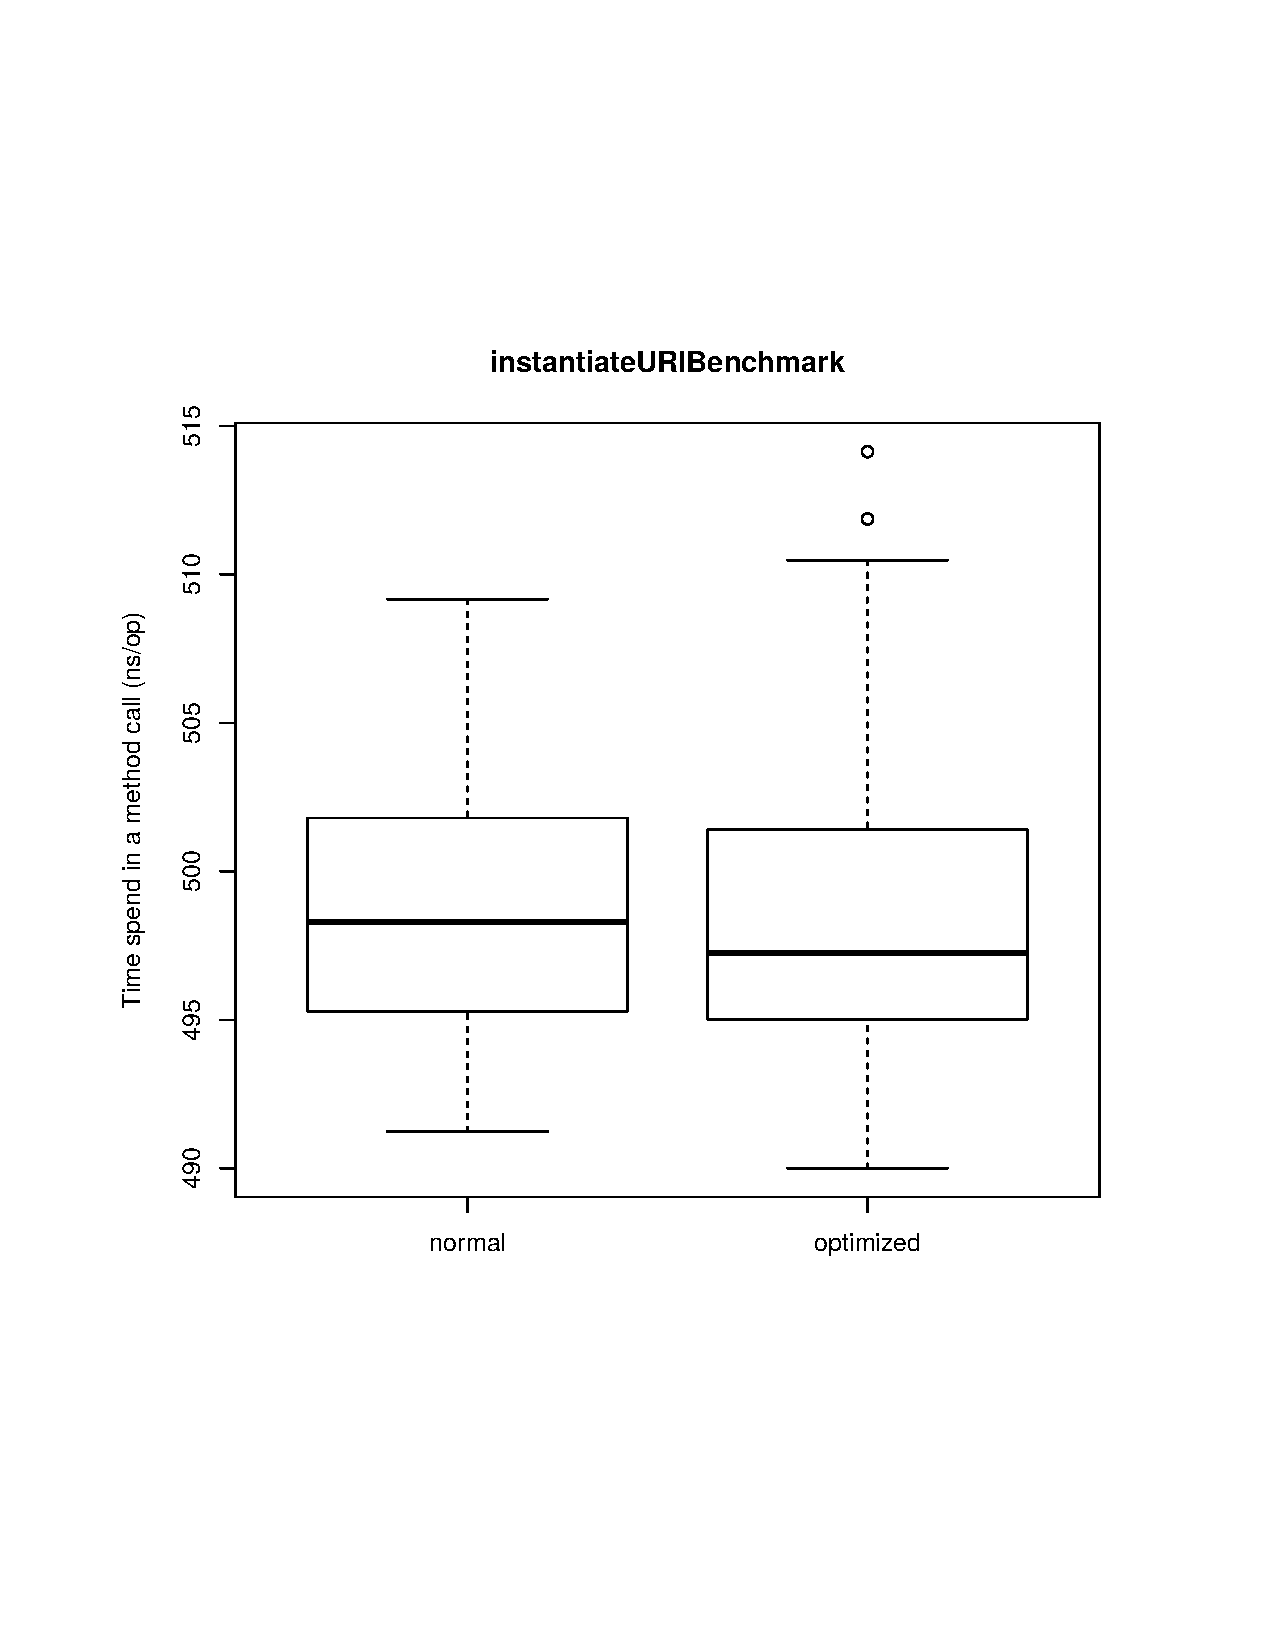
\includegraphics[trim=0mm 60mm 20mm 50mm,scale=0.50]{pictures/boxplot_instantiateURI.pdf}
		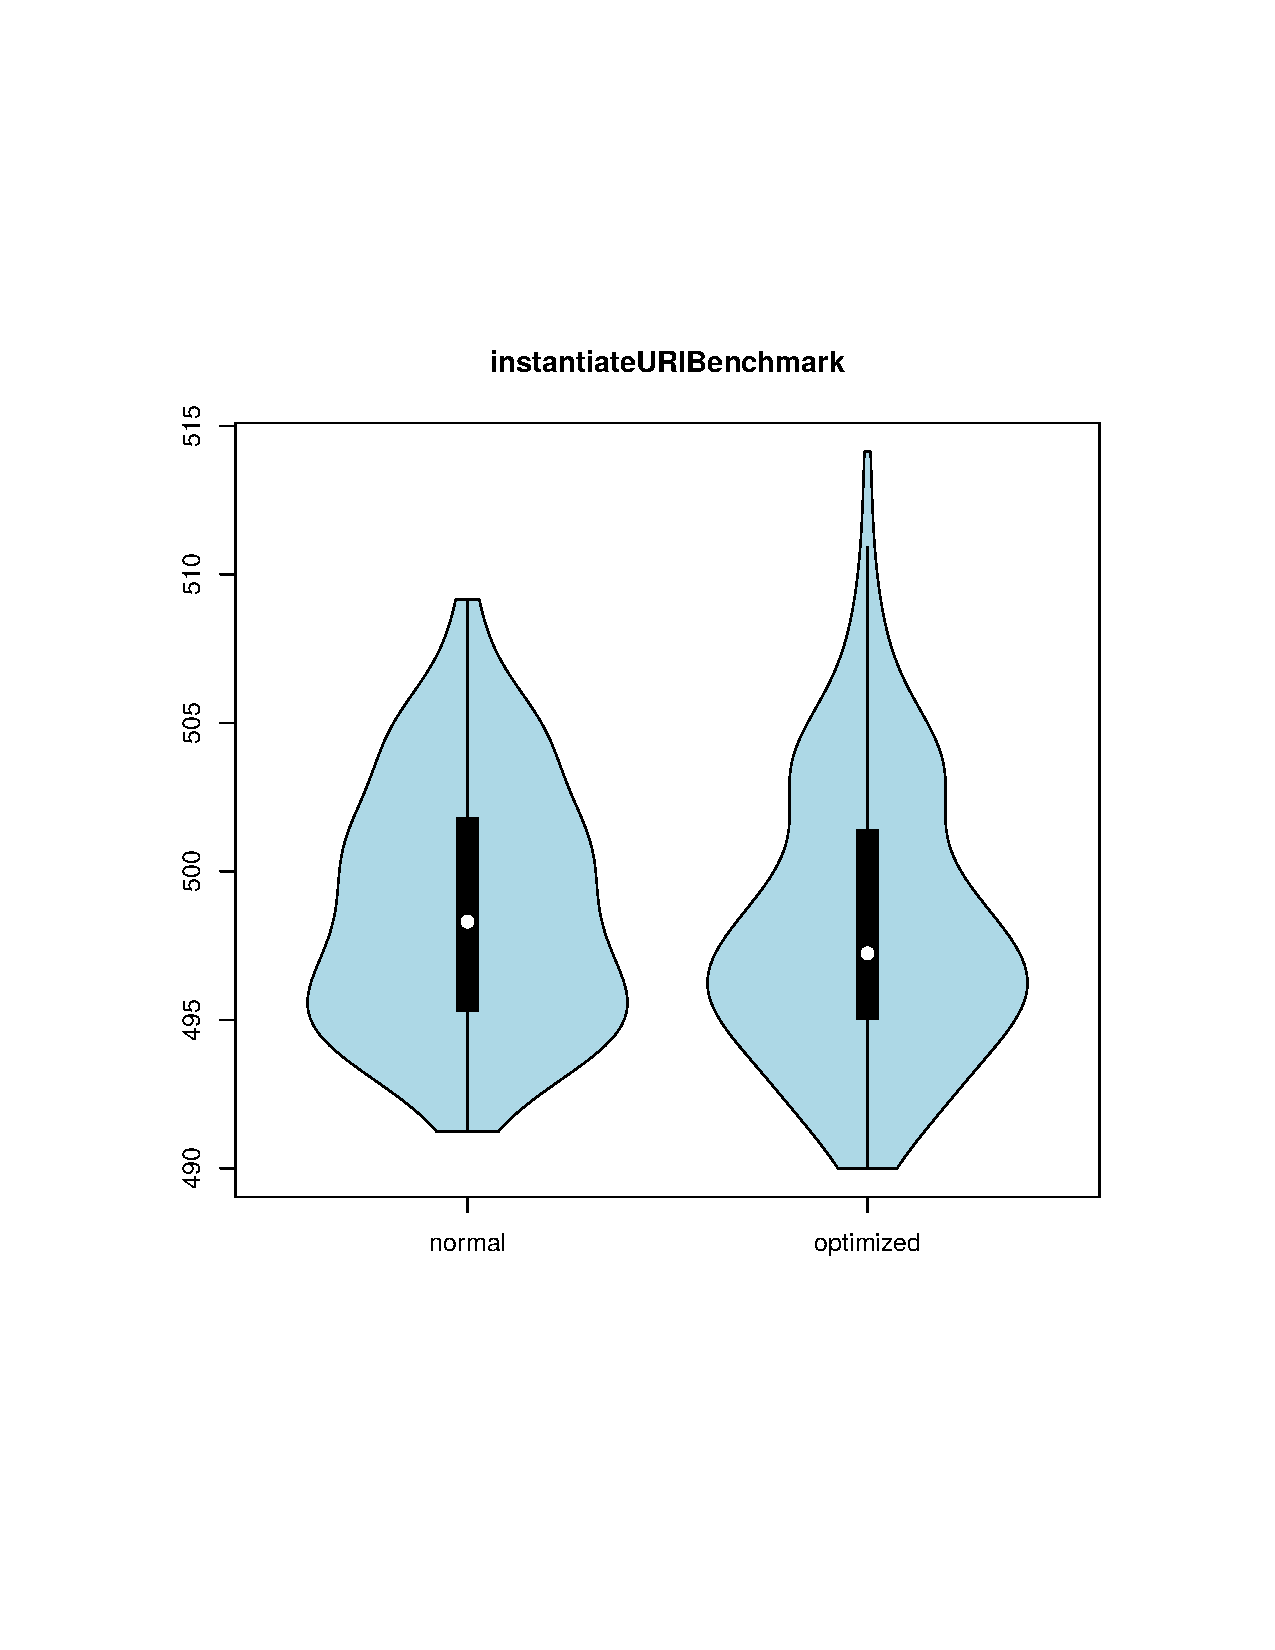
\includegraphics[trim=20mm 60mm 0mm 50mm,scale=0.50]{pictures/vioplot_instantiateURI.pdf}
	}

	\begin{table}[H]
	\centering
		\begin{tabular}{|l|r|r|r|}
			\hline
		   		 	  & Mittelwert & Median & \bf{$\pm$ $0,1\%$} \\
		 	\hline
		 	\hline
		  	normal 	  & 498,79 & 498,30 & 0,965 \\
		 	optimiert & 498,22 & 497,24 & 1.086 \\ 
		  	\hline
		  	
		\end{tabular}
	\end{table}

	\caption{Ergebnis des instantiateURI Benchmarks}\label{bp:instURIBench}
\end{figure}

\paragraph{Auswertung}

Bei der Optimierung dieser Methode stellen sich einige Probleme dar. Die zur 
Optimierung verwendete Referenz wird durch einen \texttt{trim} Aufruf auf der
übergebenen URI definiert. Diese Referenz wird innerhalb der Methode häufig benutzt
und mit jedem \texttt{substring} Aufruf auf diese Referenz wird eben diese wieder 
überschrieben. Zu den sonstigen aufgerufenen Methoden auf diesen Referenzen gehören:

\begin{itemize}
  	\item \texttt{startsWith}
  	\item \texttt{length}
  	\item \texttt{charAt} 
\end{itemize}  

Wobei \texttt{length} und \texttt{charAt} auch vom Typ \texttt{SubstringString}
implementiert werden. Darüber hinaus werden diese \texttt{SubstringString} Referenzen
an die folgenden privaten Methoden übergeben. 

\begin{itemize}
 	\item \texttt{initializeScheme(String)}
 	\item \texttt{initializeAuthority(String)}
 	\item \texttt{initializePath(String)}
\end{itemize} 

In diesen Methoden werden wiederum unter anderem \texttt{substring} Aufrufe auf 
den übergebenen String ausgeführt.

All diese anderweitigen Verwendungen der optimierten Referenz sorgen dafür, dass die
Bubble an diesen Stellen endet und eine Konvertierung zum originalen Typ 
\texttt{java.lang.String} stattfindet. Diese Konvertierungen haben allerdings negative 
Auswirkungen auf die Laufzeit, wodurch die Optimierungseffekte wieder aufgehoben werden.    

\subsubsection{xNumberToString}

Eine \texttt{org.apache.xpath.objects.XNumber} repräsentiert eine Zahl innerhalb eines
XPath Ausdrucks. Die Methode \texttt{str():java.lang.String} wandelt die intern Verwaltete
Dezimal Zahl in eine String Repräsentation dieses Wertes um. Dabei wird das Ergebnis
des Ausdrucks \texttt{Double.toString(val)}, wobei \texttt{val} der aktuelle Wert des
Objektes ist, einem String zu gewiesen. Dieser String wird daraufhin in ein alternatives
Dezimal Zahlen Format umgewandelt: 

\begin{itemize}
 	\item Es werden 'NaN' bzw. 'Infinity' Strings erzeugt
 	\item Bei Ganzzahlen wird das folgende '.0' abgeschnitten
 	\item Für Zahlen mit Exponenten werden werden diese ausgeschrieben
\end{itemize} 

Um die verschiedenen Teile der Verarbeitung innerhalb der Methode mit zu berücksichtigen 
wurde der Test mit verschiedenen Eingabe durchgeführt:

\begin{itemize}
	\item Einer positiven Dezimalzahl (12,34)
	\item Einer negativen Dezimalzahl (-12,34)
	\item Einer positiven Ganzzahl (12)
	\item Einer Zahl mit negativem Exponent (0,12e-5)
\end{itemize}

Im folgenden sind die einzelnen Testergebnisse aufgeführt. Eine Auswertung dieser
Ergebnisse folgt auf diese Darstellungen.


\begin{figure}[H]
	\centering

	\centerline{
		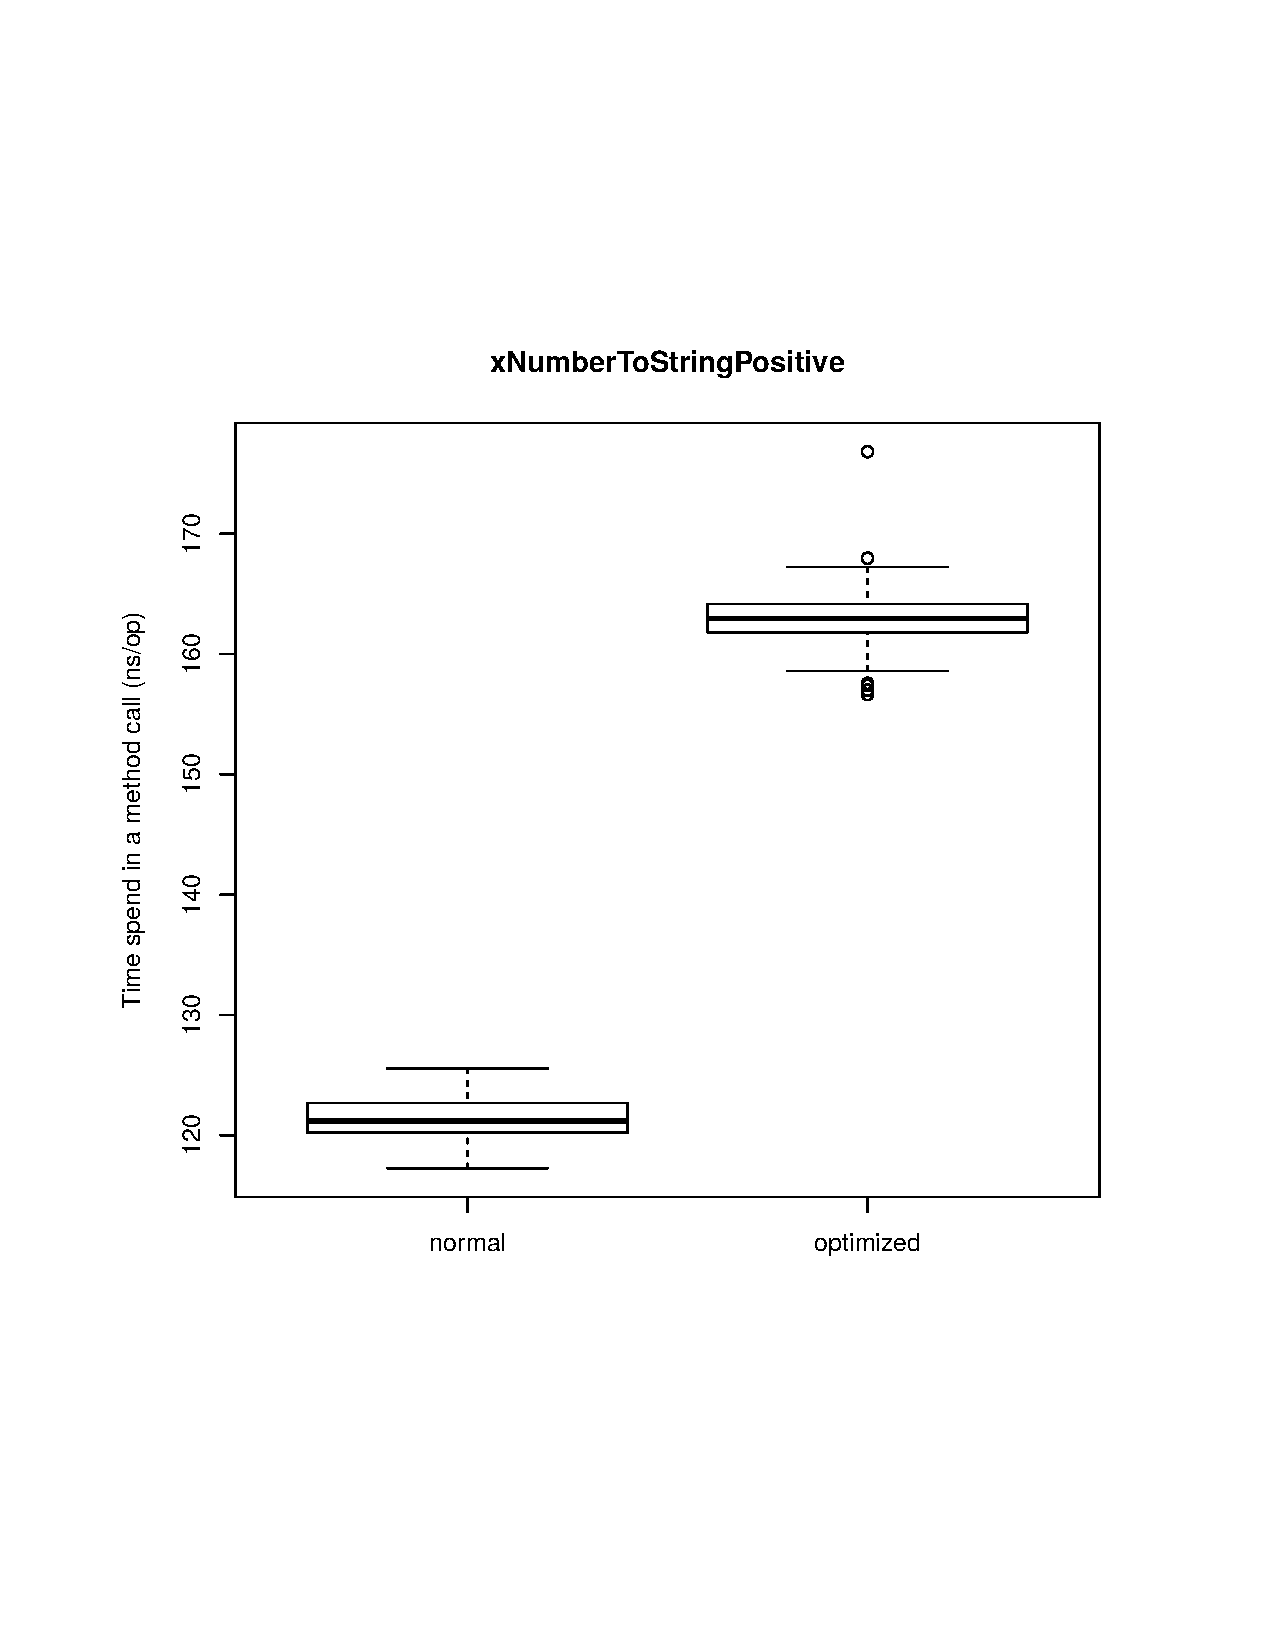
\includegraphics[trim=0mm 60mm 20mm 50mm,scale=0.50]{pictures/boxplot_xNumberToStringPositive.pdf}
		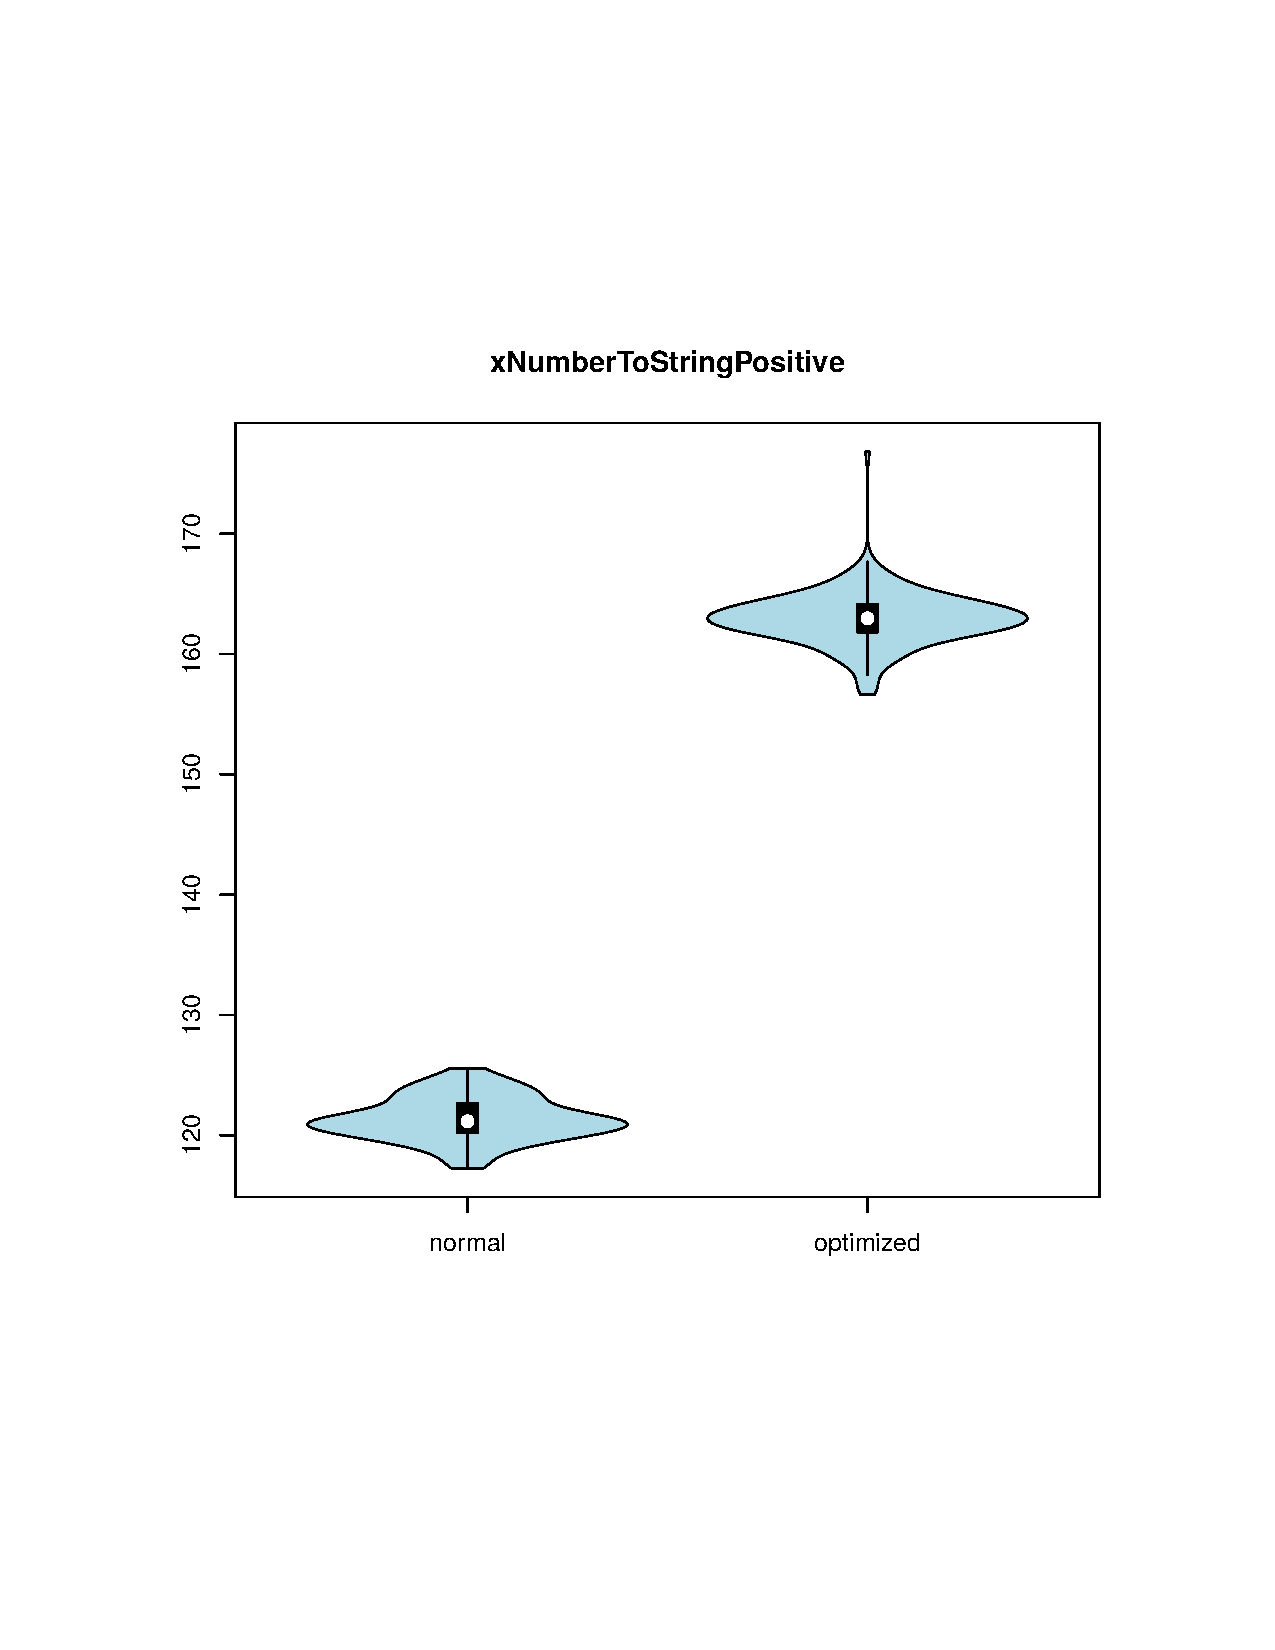
\includegraphics[trim=20mm 60mm 0mm 50mm,scale=0.50]{pictures/vioplot_xNumberToStringPositive.pdf}
	}
	\begin{table}[H]
	\centering
		\begin{tabular}{|l|r|r|r|}
			\hline
		   		 	  & Mittelwert & Median & \bf{$\pm$ $0,1\%$} \\
		 	\hline
		 	\hline
		  	normal 	  & 121,38 & 121,17 & 0,425 \\
		 	optimiert & 162,93 & 162,97 & 0,518 \\ 
		  	\hline
		  	
		\end{tabular}
	\end{table}

	\caption{Ergebnis des xNumberToString Benchmarks (positive Dezimalzahl)}\label{bp:instURIBench}
\end{figure}



\begin{figure}[H]
	\centering

	\centerline{
		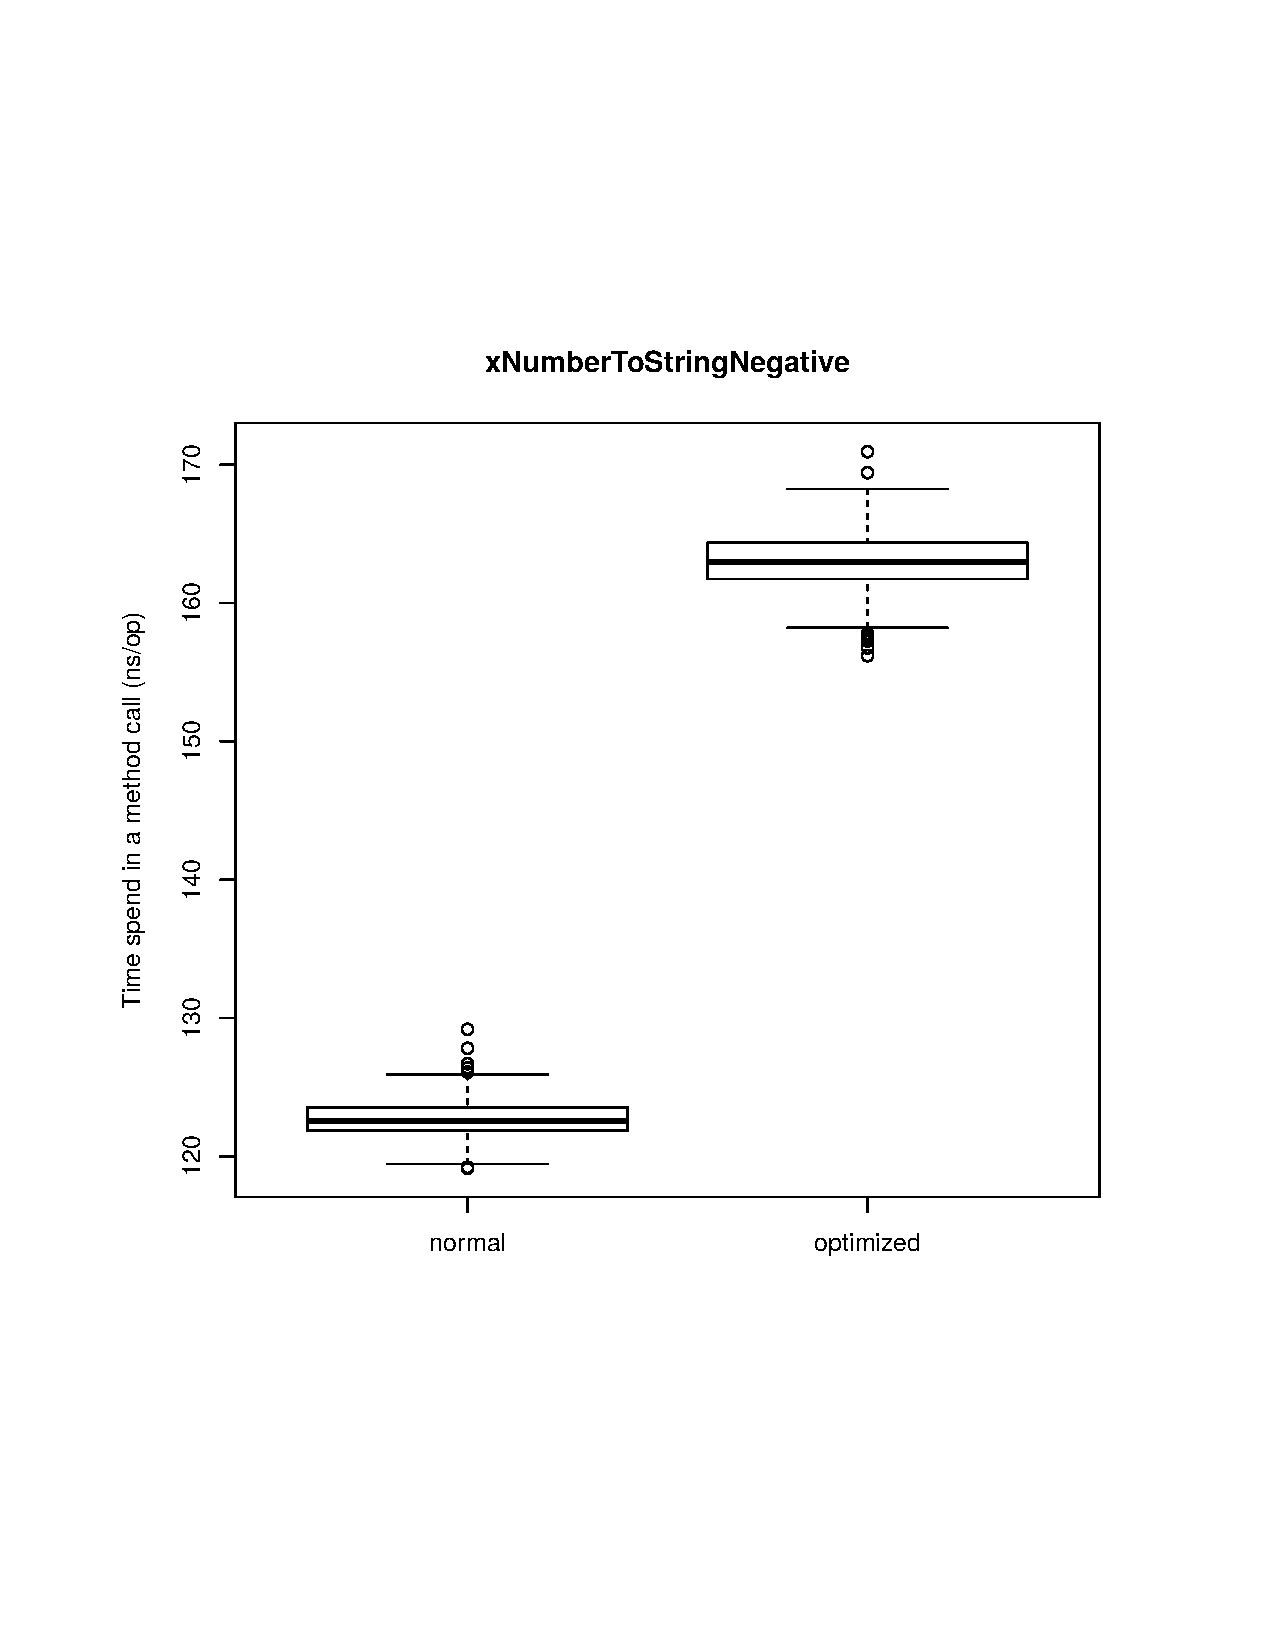
\includegraphics[trim=0mm 60mm 20mm 50mm,scale=0.50]{pictures/boxplot_xNumberToStringNegative.pdf}
		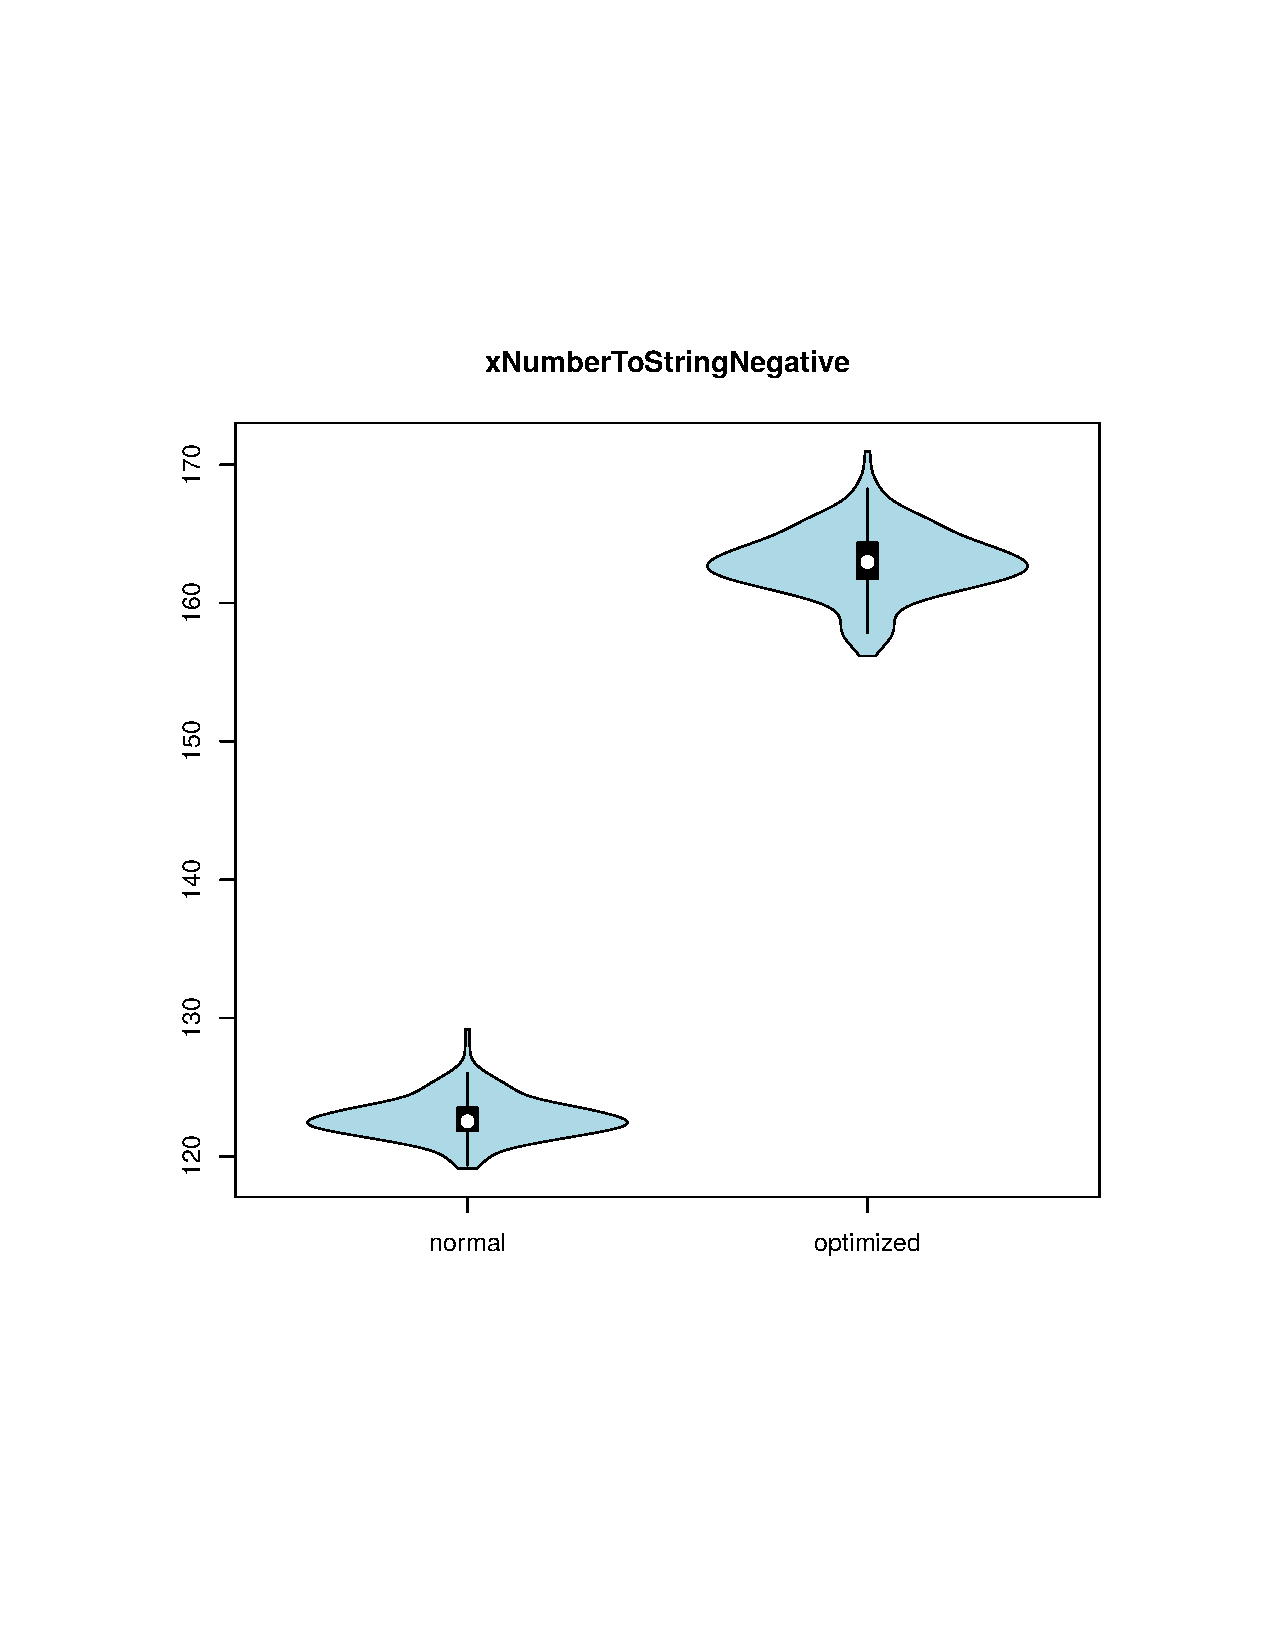
\includegraphics[trim=20mm 60mm 0mm 50mm,scale=0.50]{pictures/vioplot_xNumberToStringNegative.pdf}
	}
	\begin{table}[H]
	\centering
		\begin{tabular}{|l|r|r|r|}
			\hline
		   		 	  & Mittelwert & Median & \bf{$\pm$ $0,1\%$} \\
		 	\hline
		 	\hline
		  	normal 	  & 122,78 & 122,54 & 0,359 \\
		 	optimiert & 162,91 & 162,97 & 0,572 \\ 
		  	\hline
		  	
		\end{tabular}
	\end{table}

	\caption{Ergebnis des xNumberToString Benchmarks (negative Dezimalzahl)}\label{bp:instURIBench}
\end{figure}


\begin{figure}[H]
	\centering

	\centerline{
		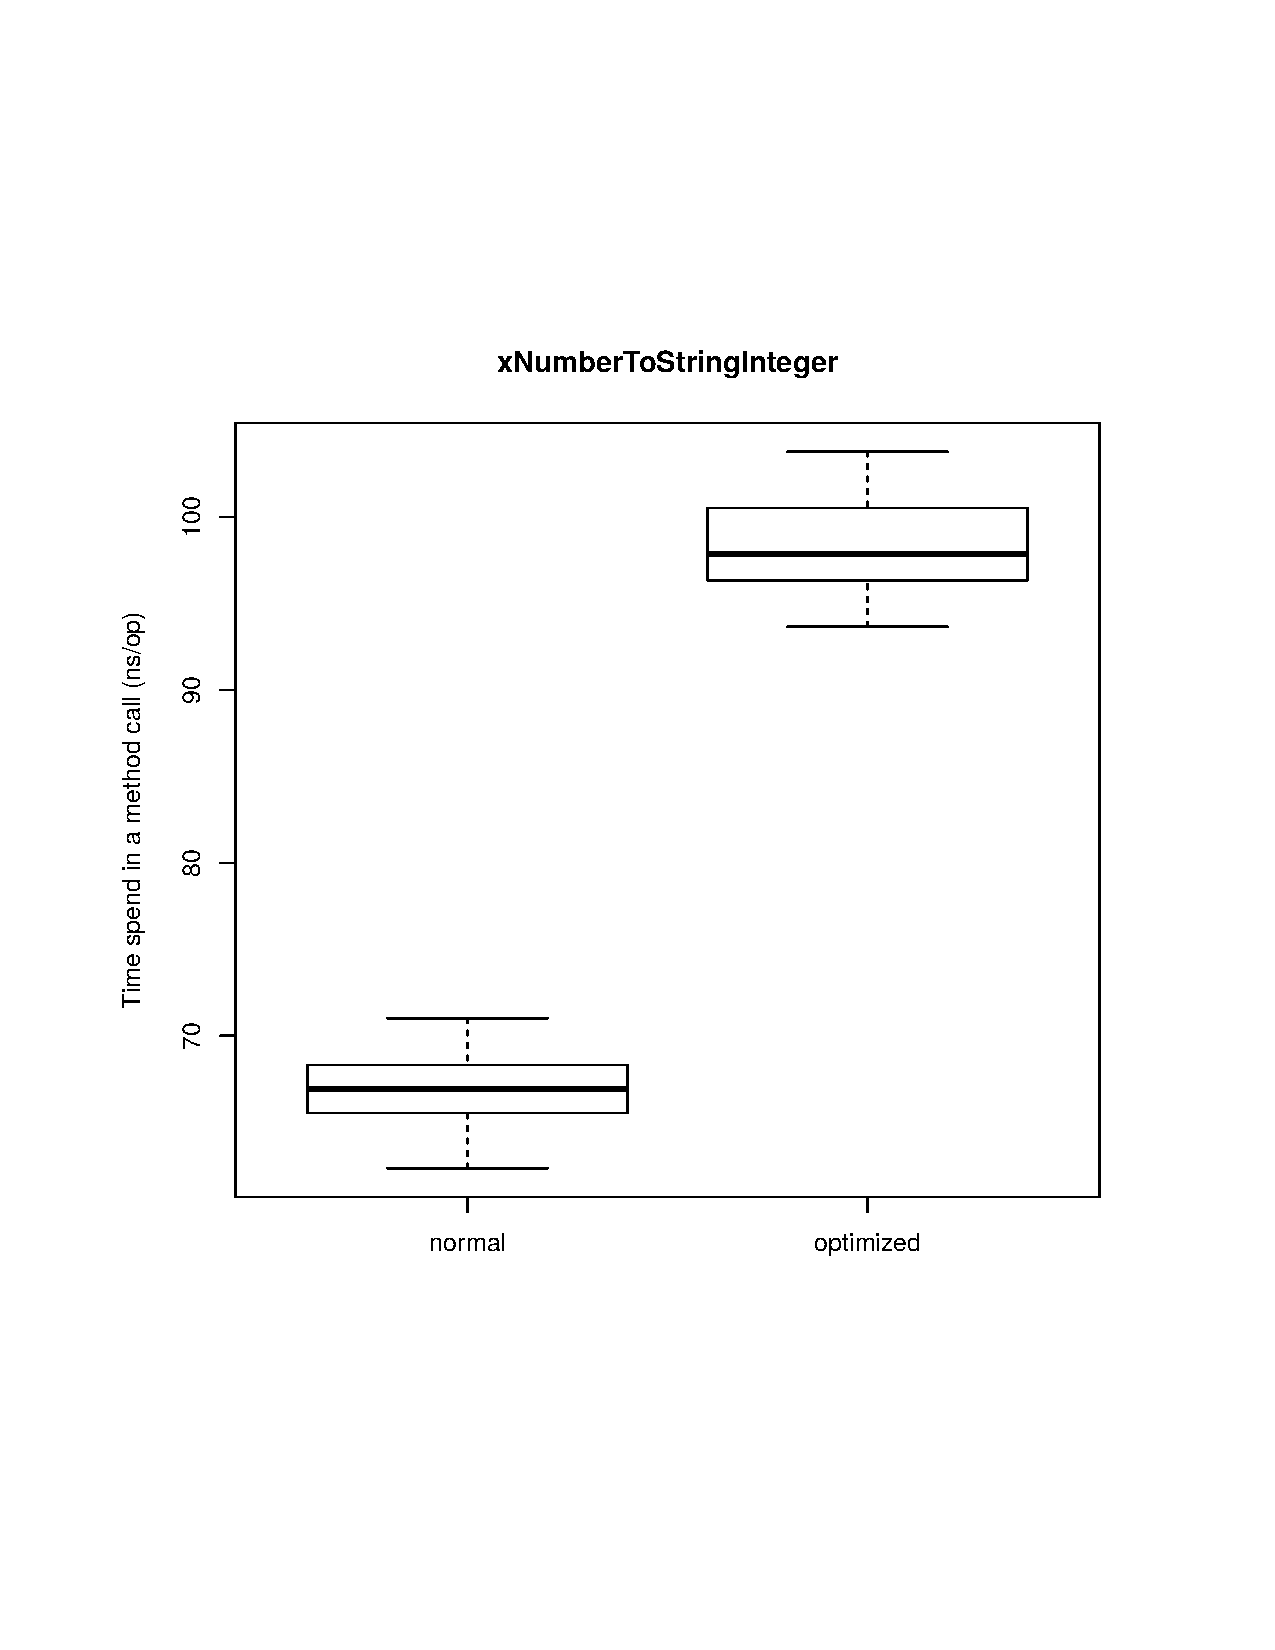
\includegraphics[trim=0mm 60mm 20mm 50mm,scale=0.50]{pictures/boxplot_xNumberToStringInteger.pdf}
		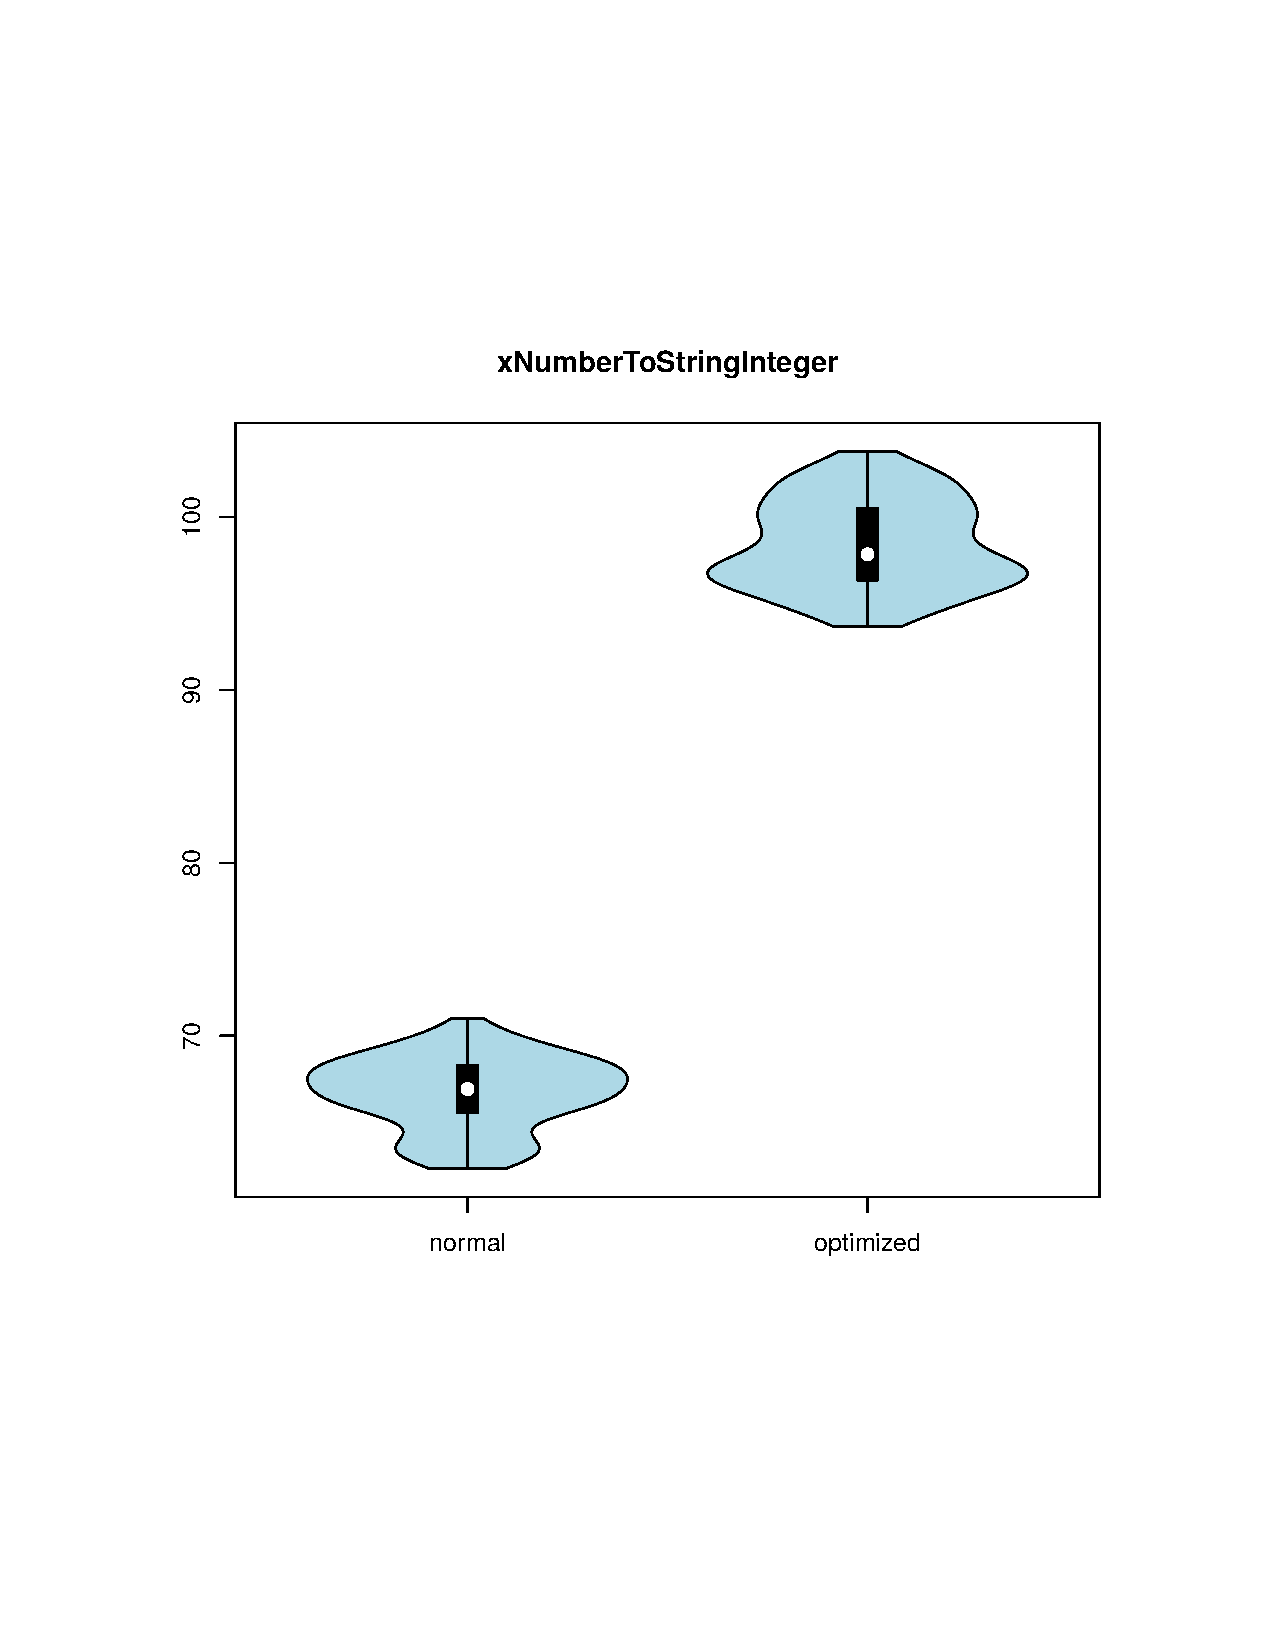
\includegraphics[trim=20mm 60mm 0mm 50mm,scale=0.50]{pictures/vioplot_xNumberToStringInteger.pdf}
	}

	\begin{table}[H]
	\centering
		\begin{tabular}{|l|r|r|r|}
			\hline
		   		 	  & Mittelwert & Median & \bf{$\pm$ $0,1\%$} \\
		 	\hline
		 	\hline
		  	normal 	  & 66,69 & 66,91 & 0,488 \\
		 	optimiert & 98,42 & 97,84 & 0,605 \\ 
		  	\hline
		  	
		\end{tabular}
	\end{table}

	\caption{Ergebnis des xNumberToString Benchmarks (positive Ganzzahl)}\label{bp:instURIBench}
\end{figure}


\begin{figure}[H]
	\centering

	\centerline{
		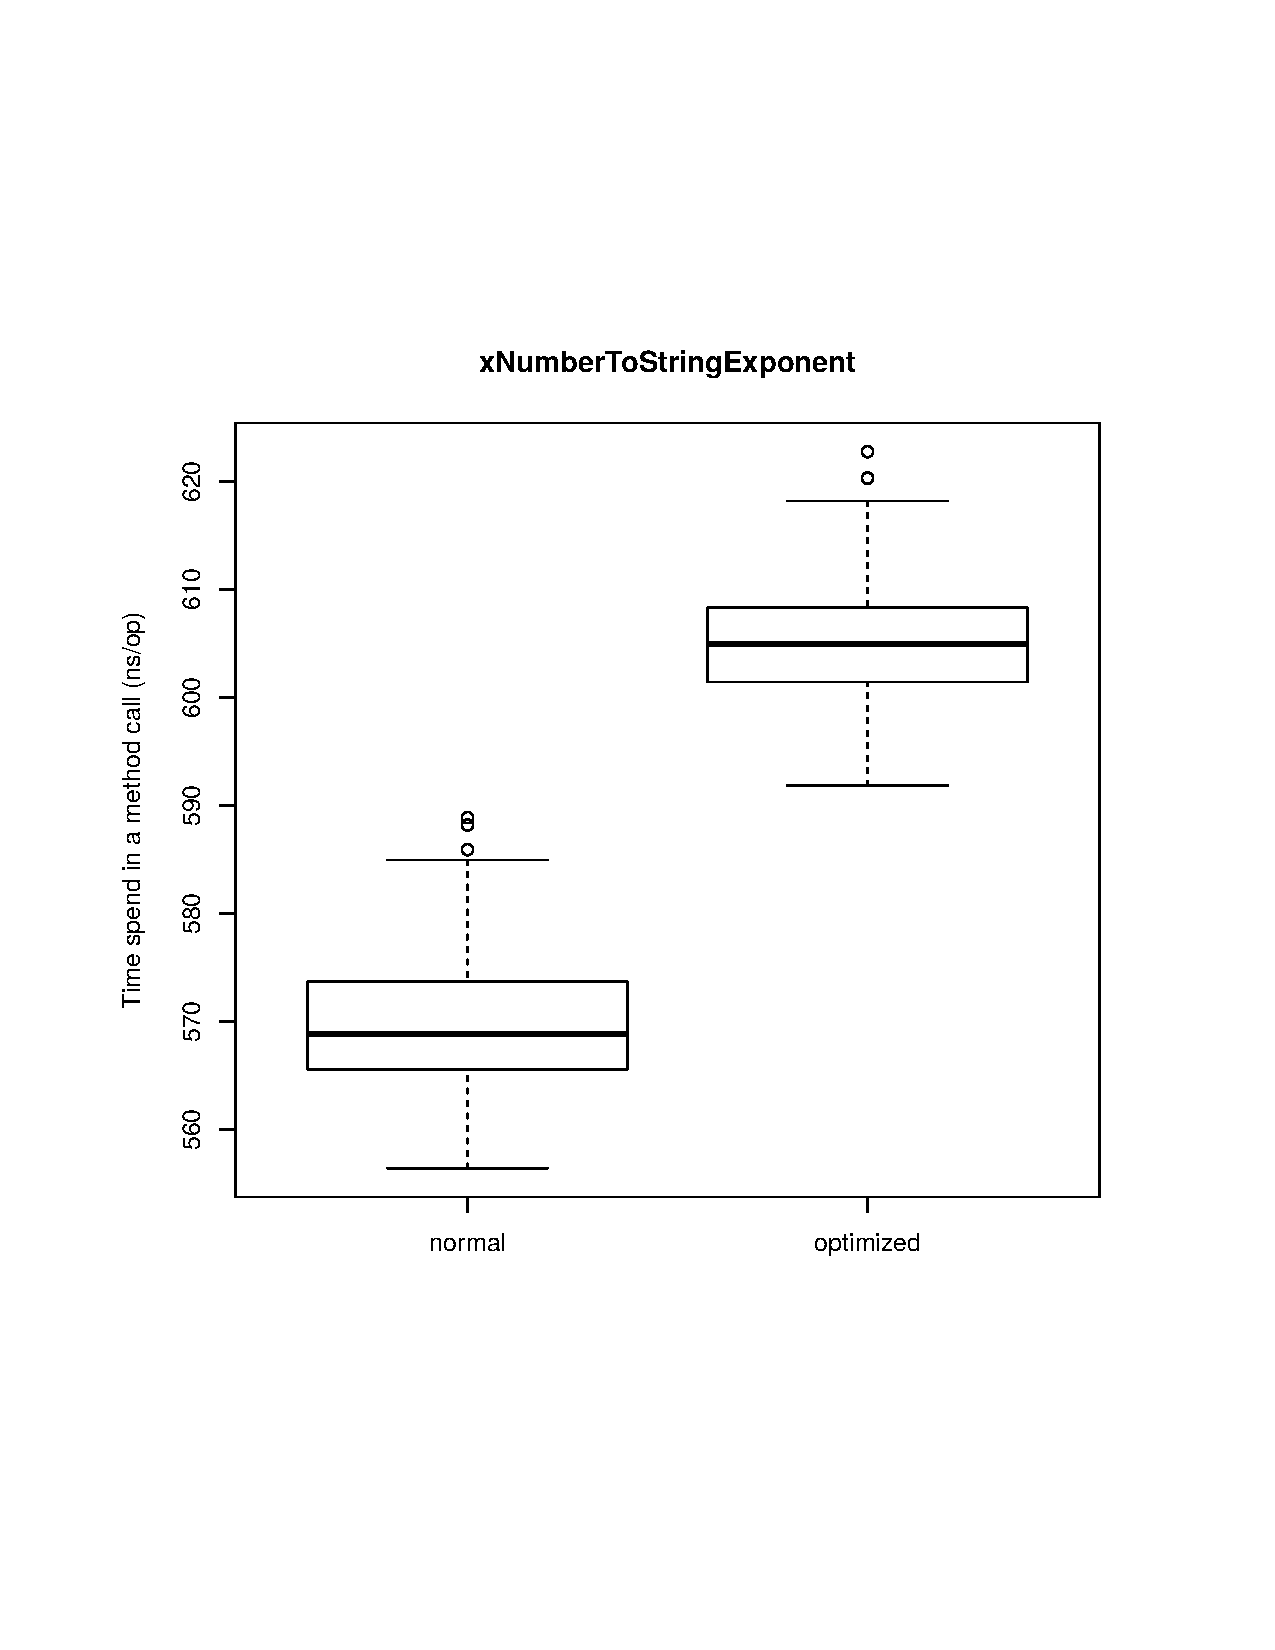
\includegraphics[trim=0mm 60mm 20mm 50mm,scale=0.50]{pictures/boxplot_xNumberToStringExponent.pdf}
		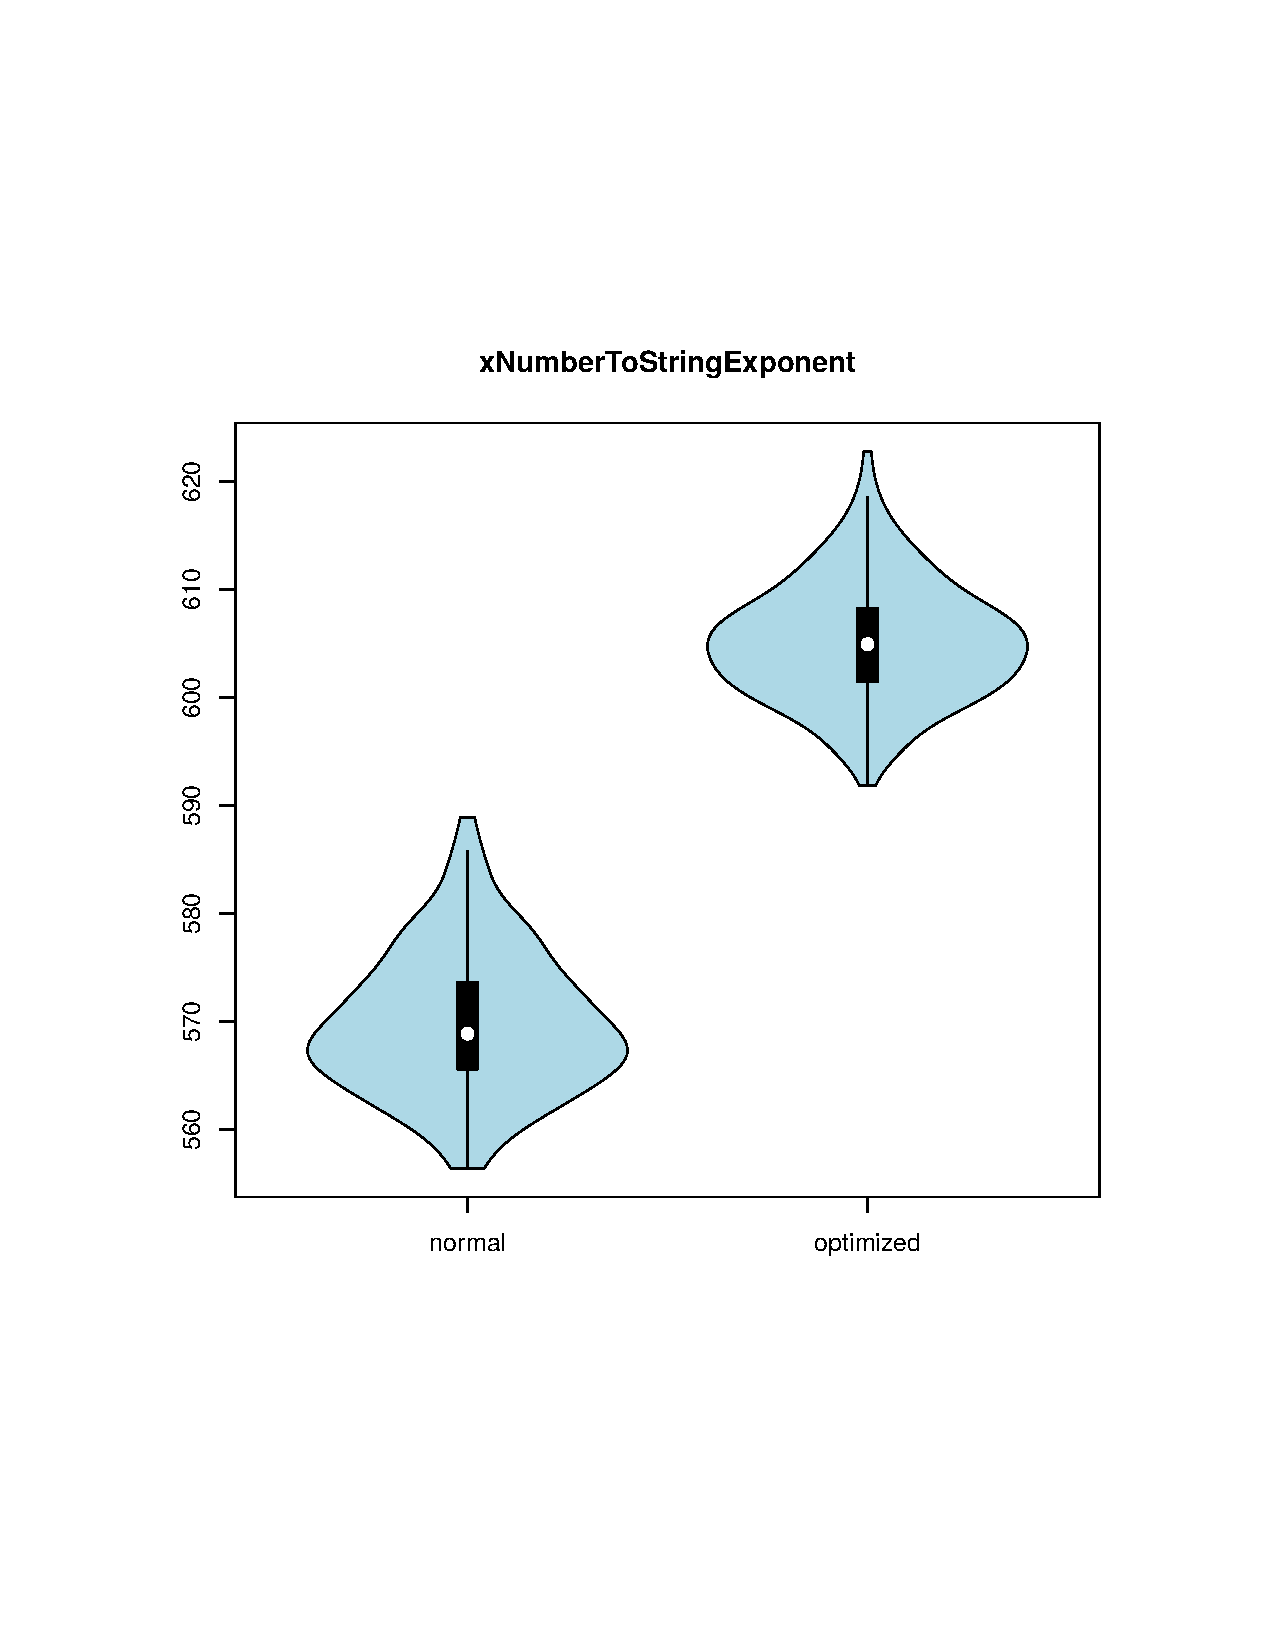
\includegraphics[trim=20mm 60mm 0mm 50mm,scale=0.50]{pictures/vioplot_xNumberToStringExponent.pdf}
	}

	\begin{table}[H]
	\centering
		\begin{tabular}{|l|r|r|r|}
			\hline
		   		 	  & Mittelwert & Median & \bf{$\pm$ $0,1\%$} \\
		 	\hline
		 	\hline
		  	normal 	  & 569,85 & 568,86 & 1.530 \\
		 	optimiert & 605,16 & 604,93 & 1,291 \\ 
		  	\hline
		  	
		\end{tabular}
	\end{table}

	\caption{Ergebnis des xNumberToString Benchmarks (positive Dezimalzahl)}\label{bp:instURIBench}
\end{figure}

\paragraph{Auswertung}

Die Implementierung dieser Methode erzeugt innerhalb der Methode eine String Repräsentation des
im Objekt verwalteten Gleitkommazahl. Dieser Wert ist vom Typ \texttt{double}. Der 
String wird über einen Aufruf von \texttt{Double.toString(double)} erzeugt, dem der 
\texttt{double} Wert der Klassen Eigenschaft übergeben wird. Diese String Referenz wird innerhalb der 
Methode formatiert. Dies geschieht über Kontrollflüsse die abhängig von der ursprünglichen Zahl sind.
Die vier Vorgestellten Benchmarks decken die verschiedenen Verarbeitungsschritte ab. Die auf der
Referenz in jedem Fall aufgerufenen Methoden (abgesehen von \texttt{substring}) sind:

\begin{itemize}
	\item \texttt{length()}
	\item \texttt{charAt(int)}
	\item \texttt{indexOf(char)}
\end{itemize}

Wobei die Methode \texttt{indexOf(char)} nicht von dem optimierten Typen unterstützt wird.
Da dieser Aufruf allerdings für jede Zahl $\neq 0$ aufgerufen wird (es wird nach dem '\texttt{e}' in
Exponenten gesucht), muss vor diesem Aufruf jeder \texttt{SubstringString} in einen String
konvertiert werden. 

Diese Konvertierungen für jeden Aufruf, zusätzlich zu denen hin zu einem \texttt{SubstringString}
und zurück zu einem \texttt{String} vor dem Zurückgeben des Strings aus der Methode, führen zu 
einer beträchtlichen Anstieg der Laufzeit in der optimierten Variante dieser Methode.


\subsubsection{compileXPath}